\documentclass[8pt]{extarticle}
\usepackage[utf8]{inputenc}
\usepackage{geometry}
\usepackage{longtable}
\usepackage{graphicx,amsmath,amsfonts,amssymb,fullpage,url,natbib}
\geometry{
 a4paper,
 margin=15mm,  % Reduced from 20mm to 15mm
 top=10mm,
 bottom=5mm,
 left=15mm,
 right=15mm,
 includeheadfoot
 }
\usepackage{graphicx}
\usepackage{titling}
\usepackage{subcaption}
\usepackage{url}
\usepackage{subcaption} 
\usepackage{hyperref}
\usepackage{float}
\usepackage{soul}
\usepackage{tcolorbox}
\usepackage{tikz}
% Optional libraries for specific functions
\usetikzlibrary{arrows,shapes,positioning,matrix,patterns}
\usepackage{tabularx}         % in your preamble
\usepackage{soul}

\usepackage{xcolor}
\usepackage{listings}
\lstset{
  basicstyle=\ttfamily\footnotesize,
  breaklines=true,
  breakatwhitespace=true
  columns=fullflexible,
  moredelim=**[is][\colorbox{blue}]{@@}{@@}
}

\title{SENTINEL: Moving Assertions Earlier for Enhanced Python Program Safety}
\author{Dinesh Vasireddy, Soham Gupta, Dhruv Patel, Lavik Jain}
% \date{March 2025}
\usepackage{natbib}
\bibliographystyle{plainnat}
\usepackage{indentfirst}

\usepackage{fancyhdr}
\fancypagestyle{plain}{%
    \fancyhf{}
    \fancyfoot[L]{\thedate}
    \fancyhead[L]{CS 2540 Final Report}}
\makeatletter
\def\@maketitle{%
  \newpage
  \null
  \vskip 1em%
  \begin{center}%
    {\LARGE \@title \par}%
    \vskip 1em%
  \end{center}%
  \par
  \vskip 1em}
\makeatother

\begin{document}

\maketitle

\begin{center}
    \theauthor
\end{center}
% \section*{Project Specification}

\section{Introduction}

Ensuring the correctness and safety of software systems often requires enforcing invariants through runtime assertions. These assertions typically appear at the end of computations, detecting violations only after resources have been consumed or side effects have occurred. This pattern is particularly common in dynamic languages like Python, where permissive semantics lead developers to write post-hoc validation logic, potentially allowing errors to propagate before detection. This raises a critical question: could violations be detected earlier in execution, before unnecessary computation occurs?

Existing approaches to this problem face significant limitations: static analysis tools struggle with Python's dynamic nature, manual refactoring is error-prone, and automated precondition inference often produces approximations that are either too strict or too lenient. The fundamental challenge lies in automatically transforming programs to detect violations earlier while preserving the exact logical guarantees of the original assertions.

We present SENTINEL, a novel approach that combines large language models (LLMs) for assertion generation with a multi-stage verification pipeline that guarantees logical equivalence between early and final checks. Our system enables more proactive error handling while maintaining program semantics. Experimental results demonstrate that early assertions can significantly reduce computational overhead (saving an average of 28.60 bytecode instructions per function) while preserving the original program's logical guarantees. We detail our motivations, results, and analysis further in the subsequent sections. 

\section{Project Overview}

This paper investigates the technical feasibility and formal verification of \textit{early assertions} which were placed earlier in program execution and are logically equivalent to existing later checks (See Figure \ref{eq:assertion-equivalence}). Our research explores how to systematically transform programs to shift violation detection earlier while ensuring transformed assertions are neither overly strict nor overly weak.

We focus specifically on Python programs, where three factors make this problem particularly challenging: (1) dynamic typing that complicates static analysis, (2) implicit type conversions that can mask potential errors, and (3) complex control flow that creates multiple execution paths. Our approach leverages recent advances in LLMs to generate candidate assertions and combines symbolic execution, fuzzing, and formal verification to validate their correctness.

The central research question we address is: \textit{\textbf{How can we generate and formally verify early assertions in Python programs that are logically equivalent to existing later checks, ensuring critical security and correctness properties are maintained and potential violations are detected proactively?}} Through our systematic evaluation across functions of varying complexity, we demonstrate both the potential and limitations of automated early assertion transformation.

\begin{figure}[H]
\centering
\begin{tcolorbox}[colback=white,colframe=black,sharp corners,boxrule=1pt,title=\textbf{Logical Equivalence of Assertions}]
For any input values $\vec{v}$ and program state $\sigma$, early assertions $\phi_{early}$ and final assertions $\phi_{final}$ must be logically equivalent:

\begin{align}
\forall \vec{v}, \sigma: \phi_{early}(\vec{v}, \sigma) \Leftrightarrow \phi_{final}(\vec{v}, f(\vec{v}, \sigma))
\end{align}

where $f$ represents the computation between early and final assertion locations.
\end{tcolorbox}
\caption{Formal definition of assertion equivalence property verified in our pipeline.}
\label{eq:assertion-equivalence}
\end{figure}

\section{Related Works}

\subsection{Enforceable Security Policies and Early Assertion Placement}
Foundational work on security policy enforcement established that certain policies can be enforced at runtime by monitoring program executions and halting before a violation occurs \cite{schneider2000}. \textbf{Schneider} formalized this notion, showing that execution monitors can insert runtime checks to stop an execution "when the security policy they enforce is about to be violated" \cite{schneider2000}. It is generally desirable to prevent execution as soon as a violation is detectable (although there are some situations in which desired computation occurs before the violation and after detection). Such inline reference monitors and runtime-checking frameworks (e.g., SASI, PoET/PSLang) demonstrated practical techniques for injecting security checks into code to enforce memory safety and access control policies at runtime. This fail-fast approach aligns with the principles of Meyer's Design by Contract, where software components check preconditions at the interface and immediately flag contract violations rather than propagate errors \cite{meyer1992}. \textbf{Meyer} introduced in the Eiffel programming language advocated that critical conditions be checked before or during execution of an operation, so that a violation is caught as early as possible, improving reliability \cite{meyer1992}.

These ideas underline our project's goal: by placing correct and equivalent assertions early in Python programs (at the point where a property can be evaluated), one can proactively detect potential correctness or security violations sooner, provided these early assertions enforce the same policy as existing late-stage checks.

% \subsection{Static and Dynamic Verification for Python}
% Fully static formal verification of Python programs is challenging due to dynamic typing and constructs. Nonetheless, recent research has produced tools that support user-specified assertions and specifications in Python. \textbf{Eilers' et al.'s Nagini paper} \cite{eilers2018} introduces a \textbf{sound static verifier for Python 3} that can prove memory safety, data race freedom, and user-supplied assertions in code. Nagini uses Mypy-style annotations and translates to the Viper intermediate verification language, supporting scalable modular reasoning. It was used to verify safety properties in production network code.

% Complementary tools like \textbf{CrossHair} \cite{CrossHairTool} offer dynamic symbolic execution in native Python. CrossHair explores feasible paths and reports concrete counterexamples. It works well with minimal annotations, but is incomplete. We employ both: using CrossHair to detect mismatches between early and final assertions, and Nagini to formally verify equivalence under full specifications.

% A related tool is \textbf{LLM-Sym} \cite{Wang2024-LLM-SymExec}, which uses LLMs to translate complex Python operations into SMT-compatible constraints, enabling symbolic execution to cover previously unsupported features such as dynamic list manipulation. While LLM-Sym improves symbolic reach, it still requires external verification to confirm semantic correctness-reaffirming our use of both dynamic and static techniques.

\subsection{Assertion Synthesis}

\subsubsection{LLMs for Assertion and Invariant Generation}

LLMs have become a common tool for assertion generation, but their approaches and guarantees vary widely. \textbf{Watson et al.} introduced ATLAS \cite{watson2020}, a neural machine translation model trained on unit test code, achieving 31\% exact matches with developer-written assertions. Recognizing its limitations with longer or uncommon assertions, \textbf{Yu et al.} \cite{yu2022} proposed a retrieval-augmented method that searches for semantically similar tests and adapts their assertions, yielding better accuracy and more interpretable outputs. While ATLAS attempts to learn general mappings, Yu's method grounds generation in past examples, making it more robust to out-of-distribution code.

Building on this idea, \textbf{Zhang et al.} \cite{zhang2024} developed RetriGen, combining a fine-tuned CodeT5 model with retrieval-based augmentation. By feeding the model both context and candidate assertions, RetriGen surpassed 57\% exact-match accuracy (which is significantly higher than prior models) and showed particular strength in longer, multi-condition asserts. Unlike Yu et al., Zhang incorporates retrieved examples into the model's input, letting it generalize more flexibly while still leveraging concrete cases.

Other directions include \textbf{Torkamani et al.} \cite{Torkamani2024-Assertify}, who use chain-of-thought prompting to synthesize inline production assertions directly from code, and further work from Zhang et al. \cite{Li2025-LLM-Assertion-Gen}, who frame assertion generation as a code-repair problem. Both rely on retrieval-enhanced prompting to boost accuracy and generalization, but mainly target postconditions.

In contrast, \textbf{Pulavarthi et al.} \cite{Pulavarthi2024-LLM-HW-Assertions} test LLMs on synthesizing formal assertions for hardware verification. They find high variability: while models generate syntactically valid assertions, correctness often suffers, especially without sufficient in-context guidance. This highlights the brittleness of unconstrained generation. \textbf{Pei et al.} \cite{Pei2023-LLM-Invariants} take a broader view, using LLMs to infer loop invariants from Java source code. Their model achieves high precision when trained on Daikon-mined datasets but struggles with pointer-heavy or structural invariants, showing the limits of purely pattern-driven learning.

While these works highlight the promise of LLMs in capturing developer intent, most focus on generating final-state or unit test assertions and evaluate success syntactically or via coverage metrics. Our work instead targets early assertion placement and enforces formal \(\phi_{early} \Leftrightarrow \phi_{final}\) equivalence. We don't just synthesize plausible assertions but prove they preserve program behavior, bridging the gap between generation and correctness.

\subsubsection{Weakest Pre-Condition Predicate Transformation}

A classical alternative to LLM-based assertion placement is \textit{weakest precondition (WP) predicate transformation}, which computes the conditions under which a later assertion would be guaranteed to hold if moved earlier in the program.

Recent work adapts WP reasoning to dynamically typed languages like Python. \textbf{Rak-amnouykit et al.}~\cite{rak-amnouykit2023weakest} perform interprocedural WP analysis to infer preconditions that prevent runtime failures (e.g., \texttt{raise} statements). Applied to libraries like \texttt{scikit-learn}, their tool generates constraints such as \texttt{penalty="elasticnet"} $\Rightarrow$ \texttt{$0 \leq l1\_\text{ratio} \leq 1$}, capturing or strengthening undocumented requirements. Their follow-up work \cite{baudart2022raise} introduces partial evaluation to simplify constraint expressions and generate machine-checkable schemas.

Other efforts apply WP-style reasoning at the specification level. \textbf{Cosler et al.}~\cite{cosler2023nl2spec} combine backward constraint propagation with LLMs to extract temporal logic specs from natural language API documentation. \textbf{Hassan et al.}~\cite{xu2018typpete} use MaxSMT-guided WP reasoning to infer interprocedural type contracts in Python via abstract interpretation.

While these techniques offer a principled way to infer sufficient preconditions, they can struggle with Python’s dynamic features—like mutable state and aliasing~\cite{guarnieri2024approximate}—and often require costly symbolic reasoning. In contrast, our method leverages LLMs to propose early assertions and then verifies their equivalence to final checks. This avoids precondition synthesis entirely and instead ensures correctness through lightweight forward reasoning and symbolic validation.

\subsubsection{Neuro-Symbolic Learning for Assertion Synthesis}
Outside of LLMs, neuro-symbolic methods have been developed to generate assertions via learning-guided search. \textbf{Si et al.} \cite{Si2018-Code2Inv} introduced \textit{Code2Inv}, which uses reinforcement learning to generate invariants with feedback from a verifier as reward. Its successor, LIPus, which was introduced in \textbf{Yu et al.} \cite{Yu2023-LIPUS}, prunes the search space and adds richer reward signals to learn more expressive invariants. \textbf{Yao et al.} \cite{Yao2020-GCLN} developed G-CLN, a logic-regression model that fits nonlinear invariant functions to execution traces. It outperformed template-based inference but was limited by the expressiveness of its features.

\subsection{Precondition Inference and Logical Equivalence Guarantees}
Ensuring that early assertions are logically equivalent to final checks is a central goal of our work. \textbf{Schneider} \cite{schneider2000} defines enforceable safety properties as those that must hold for all prefixes of execution. This principle motivates early assertion placement when violations are inevitable.

\textbf{Dinella et al.} \cite{Dinella2024-NatPrecondition} attempt to synthesize human-readable preconditions by simplifying downstream conditions and lifting them earlier in code. Their tool discovers "natural" preconditions that ensure safe execution but stops short of proving equivalence to later checks. \textbf{Menguy et al.} \cite{Menguy2022-PRECA} take a black-box approach, using constraint acquisition to learn necessary input conditions that avoid failures. Their system can infer rich safety constraints even in code with third-party calls, but the results may be overly conservative and lack formal guarantees.

\textbf{Koenig and Shao} \cite{KoenigShao2021CompCertO} offer a complementary perspective through their work on \textit{CompCertO}, a modular extension of the CompCert verified C compiler. They formally prove that source-level specifications (including pre- and post-conditions at component boundaries) are preserved across compilation, ensuring semantic correctness even in open-component settings. While their focus lies in compiler verification, the emphasis on preserving input-output behavior and component-level equivalence aligns with our goals of proving \(\phi_{early} \Leftrightarrow \phi_{final}\) after transformation. Their work reinforces the idea that transformations across compiler phases or within program execution can maintain behavioral fidelity when guided by formal specification preservation.

Unlike these works, which either approximate preconditions heuristically or verify equivalence at the compiler level, our approach targets Python programs directly, focusing on synthesizing and verifying early run-time checks. We do not infer approximations but instead construct and prove assertion equivalence through a combined pipeline of LLMs, symbolic execution, and static verification.

\subsection{Hybrid Verification: Symbolic Execution, Fuzzing, and Static Verification}

We adopt a hybrid verification strategy that integrates symbolic execution, fuzzing with random inputs, and static analysis to validate assertion correctness. Symbolic execution tools like \textbf{CrossHair} and \textbf{PyExZ3} explore feasible execution paths using SMT solvers to check satisfiability \cite{CrossHairTool, ball2015, bruni2011}. Utilizing CrossHair as a verification method, our system verifies that synthesized early assertions match final ones across all reachable paths. To complement path-based analysis, we use \textbf{Hypothesis}, a property-based fuzzing library that generates edge-case inputs.

These methods are inherently incomplete: symbolic tools suffer from path explosion and unsupported features, while fuzzing lacks formal guarantees. We address these limitations with \textbf{Nagini}~\cite{eilers2018}, a sound static verifier for Python 3 that proves user-specified assertions via modular reasoning in the Viper intermediate language. Originally used to verify safety in production network code, Nagini supports Mypy-style annotations and handles concurrency properties like memory safety and race freedom.

Our multi-layered approach reflects neuro-symbolic frameworks such as \textit{Driller}, blending broad bug exposure with formal rigor. \textbf{Liu et al.}~\cite{Liu2023-LLM-Sym-Inv} advance this further with LLM-SE, combining LLM-inferred invariants and symbolic execution analysis to outperform either method alone. Similarly, \textbf{LLM-Sym}~\cite{Wang2024-LLM-SymExec} extends symbolic execution to previously unsupported Python features, like dynamic list operations, by translating them into SMT-compatible constraints. While powerful, it still requires external validation — reinforcing the need for both dynamic and static verification layers.

\subsection{Ranking, Filtering, and Post-Processing of LLM Assertions}
Because LLM-generated assertions vary in correctness, post-processing methods help reduce verification burden. \textbf{Chakraborty et al.} \cite{Chakraborty2023-iRank} propose \textit{iRank}, a contrastive learning model trained to distinguish between provable and unprovable invariants using verification feedback. It prioritizes likely-correct invariants and improves verification throughput.

\textbf{Hellendoorn et al.} \cite{Hellendoorn2019-DAIKON-Ranking} applied similar filtering to Daikon's dynamic invariants, using ML models to predict which ones are likely to hold across executions. These rankers reduce noise and guide developers toward useful assertions. \textbf{So and Oh} \cite{SoOh2023SmartFix} extend these ideas to automated program repair, introducing a verifier-guided system called \textit{SmartFix} that accelerates the generate-and-verify loop using statistical models. Their framework filters candidate code patches by passing each through a safety verifier, retaining only semantically correct fixes. While their domain focuses on smart contract repair, the core methodology, leveraging verification feedback to select high-confidence candidates, parallels the challenge of filtering LLM-generated code. Unlike purely syntactic or heuristic methods, SmartFix incorporates semantic validation to ensure output correctness, aligning with our goals of verification-informed selection of early assertions.

While we do not use a learning-based ranker, our pipeline acts as a verification filter: only assertions that pass equivalence checks are accepted. Nonetheless, iRank- or VERSE-style models could complement our approach by prioritizing candidate assertions before verification, reducing tool burden and guiding LLM output quality—especially when integrated with retrieval-augmented generation.

% These methods emphasize the promise of hybrid learning + verification strategies. Our project follows this direction: letting LLMs propose early conditions and verifying them through formal means. The key distinction is that we operate at the level of assertion placement and equivalence checking — not general invariant mining.


\section{Methodology}
\subsection{Overview}
% Our goals are to (1) ensure logical equivalence in shifted runtime assertion checks (2) proactively enforce security and correctness properties, and (3) avoid unnecessary execution and computation. 

Our goal is to proactively enforce security and correctness properties (and prevent unnecessary computation) in Python programs by shifting runtime assertion checks earlier in execution, while ensuring that the new early assertions are \textit{logically equivalent} to the original final assertions. To achieve this, we design a three-phase pipeline that combines LLMs, program transformation, and formal verification methods. This methodology allows us to generate proposal transformations and validate their accuracy.

\begin{enumerate}
    \item \textit{Assertion Generation:} Use a large language model (GPT-o3-mini) to generate candidate early, equivalent assertions (\(\phi_{early}\)) in specified locations (that are earlier in the program) based on program context and the existing final assertion (\(\phi_{final}\)). We also provide the LLM context using condensed forms of wikis on Python assertion generation and best practices for ensuring logical consistency when making program modifications.  
    % As context, we provided the LLM with articles on best practices to generating assertion statements early in programs, see [] and [].
    \item \textit{Program Transformation:} Create a "transform program" that introduces boolean variables \(b_{early}\) and \(b_{final}\) representing \(\phi_{early}\) and \(\phi_{final}\), respectively, and asserts \(b_{early} == b_{final}\) to encode logical equivalence of the early and final checks. For programs with multiple assert statements, this boolean representation and combined assert would involve more variables and equivalence checks. See Figure \ref{fig:example-program}. 
    \item \textit{Testing \& Verification Pipeline:} We then apply testing \& formal methods on the transform program to verify that the LLM-added early assertion(s) enforce the same properties as the existing later assertions.

    \begin{itemize}
        \item \textbf{Symbolic Execution:} Employ CrossHair to explore execution paths of the transform program, searching for counterexamples where \(b_{early}\) and \(b_{final}\) differ.
        \item \textbf{Fuzz Testing:} Systematically generate random and boundary-case inputs designed to violate assertions, confirming that no input triggers a mismatch between early and final assertions.
        \item \textbf{Static Verification:} Apply Nagini to formally prove that for all inputs and execution paths, \(\phi_{early} \Leftrightarrow \phi_{final}\), discharging verification conditions automatically.\textit{*Nagini is experimental and doesn't support a variety of program features, so we only apply this step for programs with supported features. }
    \end{itemize}
\end{enumerate}

\begin{figure}[H]
\scriptsize
\setlength{\tabcolsep}{4pt}
\renewcommand{\arraystretch}{1}
\begin{tabular}{|p{0.31\linewidth}|p{0.31\linewidth}|p{0.31\linewidth}|}
\hline
\textbf{Input Python Program} & \textbf{LLM‑Altered Program} & \textbf{Transformation Program} \\
\hline
\begin{lstlisting}
def process_data(x: int):
    @@ [insert earlier assert here]
    y = x * 2
    if y > 0:
        z = y
    else:
        z = -y
    assert z == 100
\end{lstlisting}
&
\begin{lstlisting}
def process_data(x: int):
@@  assert x == 50
    y = x * 2
    if y > 0:
        z = y
    else:
        z = -y
    assert z == 100
\end{lstlisting}
&
\begin{lstlisting}
def process_data_transformed(x: int):
    b_early = (x == 50)
    y = x * 2
    if y > 0:
        z = y
    else:
        z = -y
    b_final = (z == 100)
    
    # Assert that early & final are equivalent
@@  assert b_early == b_final
\end{lstlisting}
\\
\hline
\end{tabular}
\caption{Example Input Program, LLM Assertion, and Transformation Program}\label{fig:example-program}
\end{figure}

\subsection{Evaluation \& Measuring Success}
\subsubsection{Primary Pipeline}

We're \textbf{evaluating our ability to successfully \textit{transform} and \textit{verify} Python programs by adding early assertions} that are equivalent to existing final assertions. We see success as \textbf{achieving upwards of 80\% success in creating verified and equivalent programs} with earlier assertions \textbf{across programs of varying difficulty.} However, even for failed transformations, we also consider \textbf{finding failure paths with high explainability} as a success of our approach and thus we evaluate that as well. For each program analyzed, we classify the result into one of three categories shown in Figure \ref{fig:program-classification} below. 
% \begin{itemize}
%     \item \textbf{Verified}: The program passes all three stages—symbolic execution, fuzz testing, and static verification—without detecting inconsistencies.
%     \item \textbf{Validated}: The program passes both symbolic execution and fuzz testing, but static verification is either inconclusive or not applicable.
%     \item \textbf{Rejected}: At least one stage produces a counterexample or fails to establish the equivalence between the early and final assertions.
% \end{itemize}

\begin{figure}[H]
\centering
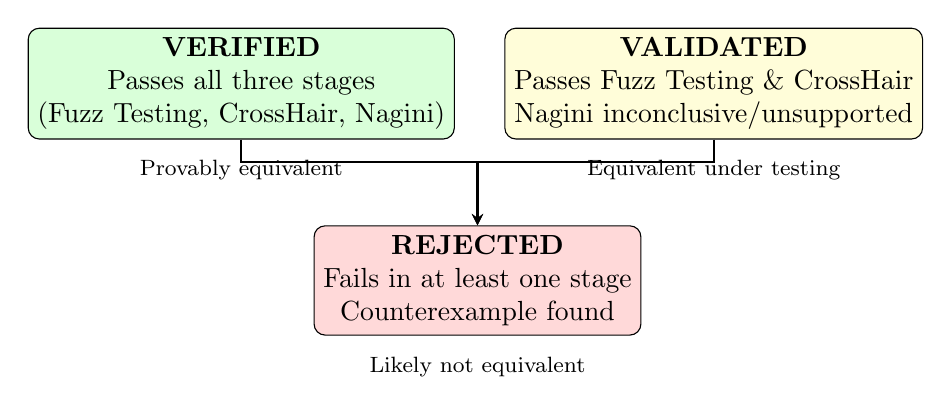
\begin{tikzpicture}[
    box/.style={rectangle, draw, rounded corners, minimum width=4cm, minimum height=1cm, align=center},
    arrow/.style={-stealth, thick}
]

% Classification boxes
\node[box, fill=green!15] (verified) at (0,0) {\textbf{VERIFIED}\\Passes all three stages\\(Fuzz Testing, CrossHair, Nagini)};

\node[box, fill=yellow!15] (validated) at (6,0) {\textbf{VALIDATED}\\Passes Fuzz Testing \& CrossHair\\Nagini inconclusive/unsupported};

\node[box, fill=red!15] (rejected) at (3,-2.5) {\textbf{REJECTED}\\Fails in at least one stage\\Counterexample found};

% Arrows
\draw[arrow] (verified) -- ++(0,-1) -| (rejected);
\draw[arrow] (validated) -- ++(0,-1) -| (rejected);

% Criteria labels
\node[align=center] at (0,-1.1) {\footnotesize Provably equivalent};
\node[align=center] at (6,-1.1) {\footnotesize Equivalent under testing};
\node[align=center] at (3,-3.6) {\footnotesize Likely not equivalent};

\end{tikzpicture}
\caption{Classification of programs after transformation and verification.}
\label{fig:program-classification}
\end{figure}

This evaluation ensures that only \textbf{ early statements that are provably equivalent} \textbf{or validated through extensive testing} \textbf{are accepted}. To support this, we define a structured process for evaluating the pipeline across diverse Python programs, sourced from open-source code, algorithm textbooks, and hand-crafted examples. Each program is annotated with metadata including line count, number of functions, control flow complexity (e.g., conditionals, loops, recursion), and data structure usage.  

% We \textbf{assign each program a difficulty rating (1–10)} based on these features. The full pipeline—from assertion generation to verification—is applied to each program, and we log equivalence results, failure stages, and verification time. We explain the particular implementation details in the subsequent section. 

Using this information, each program is systematically assigned \textbf{a difficulty rating (1-5)} after being evaluated on nine weighted components detailed in Table \ref{tab:difficulty-rating}. The scoring system applies specific scaling factors for each component to enable consistent evaluation of function difficulty and help identify correlations between program complexity and failure explanation quality (see Table \ref{tab:difficulty-rating} below). The weights were established through over 50 iterations of tuning using data from 120 benchmark programs, where each metric's weight was adjusted to maximize correlation with difficulty ratings from 5 expert annotators and performance slowdowns in 3 static analyzers; metrics like control flow depth (0.70) and loop complexity (0.60) received higher weights due to their strong, consistent impact on reasoning complexity observed across both human assessments and tool behavior in early testing.


\begin{table}[H]
\centering
\begin{tabular}{|l|c|}
\hline
\textbf{Parameter} & \textbf{Weight} \\
\hline
Parameter Complexity         & 0.30 \\
Operation Density            & 0.40 \\
Assertion Count              & 0.20 \\
Control Flow Depth           & 0.70 \\
Data Type Diversity          & 0.25 \\
Assertion Complexity         & 0.80 \\
Mathematical Sophistication  & 0.50 \\
Loop Complexity              & 0.60 \\
Function Call Density        & 0.35 \\
Branching Complexity         & 0.50 \\
Bytecode Complexity          & 0.45 \\
\hline

\end{tabular}
\caption{Complexity Metrics and Weights (matching implementation)}
\label{tab:difficulty-rating}

\end{table}
\subsubsection{Explaining Failures}
For \textbf{rejected and not verified transformations}, we introduce a \textbf{Failure Explanation Quality (FEQ) score (0-1)} that measures counterexample specificity, diagnostic clarity, and actionability of the failure information. We evaluate the stack traces, failure logs, discovered counterexamples, and conditions from failed executions on Hypothesis, CrossHair, and Nagini. This provides an additional metric to evaluate our verification pipeline's effectiveness even when assertions are incorrect or transformations fail, with a target average FEQ score of 0.5 or higher across all failed cases being preferred. Our scoring system assesses failure messages using four weighted criteria detailed in Equation \ref{eq:feq}.

\begin{equation}
\label{eq:feq}
\text{FEQ} = 0.3 \cdot S_{\text{spec}} + 0.3 \cdot S_{\text{action}} + 0.2 \cdot S_{\text{context}} + 0.2 \cdot S_{\text{tech}}, \quad
\begin{cases}
S_{\text{spec}} = \text{specificity} \\
S_{\text{action}} = \text{actionability} \\
S_{\text{context}} = \text{context} \\
S_{\text{tech}} = \text{technical detail}
\end{cases}
\quad \text{where all } S_i \in [0,1]
\end{equation}

Ultimately, we aim to evaluate the \textbf{feasibility of automatically generating and verifying equivalent early assertions in Python programs} across a diverse set of real-world examples. While conducting FEQ evaluations, we also identify \textbf{\textit{false positives}} where \textbf{assertions are deemed not equal due to a non-logical error} with the method, an unsupported feature, type errors, etc. In this case, the assertion equivalence for that method would be deemed inconclusive. 

\subsection{Practical Implementation} 

We evaluated the pipeline on 50 Python functions, each implementing basic arithmetic, complex control flow, or structural operations such as multiplication, discount calculation, factorial calculation, sine function, and data transformation. These functions span operations from basic mathematical computations to complex string processing and data transformations. We also developed automated scripts to synthesize early assertions and transform programs, computed difficulty metrics, ran testing and verification, and generated failure‑explanation scores for each program. In particular, we \textbf{identified Nagini-unsupported programs using GPT-4.1} (with Nagini's wiki as context) to assess compatibility with its specification language, followed by manual verification \cite{eilers2018}. We also used a similar LLM-as-a-judge approach to score failures across all methods to calculate Failure Explanation Quality (FEQ) scores and false positives. 

\subsubsection{Adaptations for Testing \& Verification Methods}
\paragraph{Hypothesis Testing.} Using the Hypothesis property-based testing framework, we executed each transformed program over 20 randomized and edge-case inputs. The transformed programs encode early (\(\phi_{early}\)) and final (\(\phi_{final}\)) assertions as boolean expressions and assert their equivalence. Our implementation uses Hypothesis's \textit{@given} decorator with appropriate strategy generators tailored to each function's domain (integers, floats, ranges). We configured testing parameters with \textit{@settings($max\_examples=20$)} to limit test cases while maintaining sufficient coverage. Each test function wraps the transformed program in a try-except block to cleanly capture and report assertion failures. For numerical functions involving floating-point calculations, we employed $st.floats()$ with carefully selected boundaries. The framework effectively demonstrates assertion equivalence in practice by encountering fewer failures than symbolic execution, highlighting the complementary nature of dynamic testing versus static verification approaches.

\paragraph{Symbolic Execution.}  

We ran CrossHair symbolic execution on each of the transformed programs. The transform programs are written to disk files with special docstring contracts using pre: and post: annotations that CrossHair understands. Our implementation captures both the early and final assertion conditions as boolean variables ($b_{early}$ and $b_{final}$) and explicitly checks for their equivalence. The code includes carefully defined preconditions that establish reasonable bounds for input variables (e.g., $-1000 \leq x \leq 1000$) to constrain the search space while ensuring comprehensive verification. Postconditions formally express the property that early and final assertions should be logically equivalent. The implementation invokes CrossHair through a subprocess call, captures its output, and reports any counterexamples found. 

\paragraph{Nagini Static Verification.} For transformed programs with supported features, we use \textbf{Nagini} to formally verify the logical equivalence $\phi_{\text{early}} \Leftrightarrow \phi_{\text{final}}$. Built on the Viper intermediate verification language, Nagini supports PEP 484-style type annotations and permission-based heap access control, but imposes strict constraints: programs must be statically typed and avoid dynamic features like \texttt{eval} or runtime field creation. Adapting programs for Nagini required \textbf{adding type annotations and contracts, minimally reformatting control flow, and eliminating unsupported language features}. Our verification process follows a two-phase strategy: first testing the original program with dynamic and symbolic methods, then adapting it for Nagini while preserving logical structure. This approach enables us to distinguish between true semantic failures (indicating assertion inequivalence) and compatibility issues (reflecting tooling limitations rather than transformation failures). 

\begin{figure}[H]
    \centering
    \begin{subfigure}[c]{0.5\linewidth}
        \centering
        \includegraphics[width=\linewidth]{crosshair-annotations.png}
        \caption{Transform Program with Cross Hair Annotations}
        \label{fig:cross-hair-annotations}
    \end{subfigure}%
    \hspace{0.05\linewidth}
    \begin{subfigure}[c]{0.3\linewidth}
        \centering
        \includegraphics[width=\linewidth]{nagini-specification-example.png}
        \caption{Transform Program in Nagini Specification Language}
        \label{fig:nagini-annotations}
    \end{subfigure}
    \caption{Annotation Examples in CrossHair and Nagini}
    \label{fig:annotation-comparison}
\end{figure}


\section{Results}

\subsection{Assurance Coverage}

Of the 50 target functions, 5 (10\%) are \emph{Verified}; 30 (60\%) are \emph{Validated}; and 11 (22\%) are \emph{Rejected} (Detailed results in Table \ref{tab:program-results}). Notably, the Verified group is dominated by pure-arithmetic functions with minimal control flow, likely contributing to their success across all three methods, whereas functions that rely on randomness, floating-point operations, or complex stdlib calls appear exclusively in the Rejected category (See Table \ref{tab:code-structure-impact}). \textit{All relevant code, figures, and tables with results are in this paper's Appendix.}

\subsection{Fail-Fast Security Impact}

Moving assertions earlier in the program yields tangible security and efficiency benefits. Across our benchmark, early assertion placement saved an average of 28.6 Python bytecode instructions per function (median 20), with over 80\% of failed inputs halted within the first 10 instructions (Figure \ref{fig:bytecode-load}). This reduction in executed instructions before error detection directly shrinks the window for side-effects, resource exhaustion, or side-channel leakage. The greatest savings were observed in pure arithmetic and simple loop functions, which typically halt in under 15 instructions, while string manipulation and floating-point operations required more computation before reaching the assertion. These results highlight the practical value of fail-fast enforcement, especially in security-sensitive or resource-constrained contexts.

\subsection{Complexity vs. Verifiability}

Verification success rates are strongly tied to program complexity. As shown in Figure \ref{fig:diff-scores-correlation}, functions with overall difficulty scores below 2.5 passed CrossHair over 80\% of the time and Nagini over 40\%, while those with scores above 4.0 rarely succeeded under either tool. The average difficulty of Verified functions was 2.0, compared to 2.7 for Rejected ones (Table \ref{tab:difficulty-sub-scores}).

To further quantify these trends, we analyzed the correlation between difficulty subscores and verification outcomes (Table~\ref{tab:diff-subscores-correlation}). For CrossHair, control flow depth (0.22) and operation density (0.08) showed weak positive correlations, indicating symbolic execution is only mildly affected by these factors. Nagini exhibited strong positive correlations with operation density (0.82) and assertion complexity (0.45), likely because programs with more explicit operations and assertions align better with static verification. Fuzzing was largely insensitive to these metrics, with the largest effect being a negative correlation with control flow depth (--0.38), suggesting only highly complex control structures reduce fuzzing success. Overall, static and symbolic tools are more sensitive to program structure than fuzzing.

A closer look at the rejected functions (Table \ref{tab:program-results}) reveals several recurring patterns. Nearly all rejected cases feature at least one of: deep or nested control flow (e.g., multiple loops or branches), floating-point arithmetic, or use of randomness and non-deterministic library calls. For example, functions like \texttt{binary\_search\_iterations}, \texttt{matrix\_determinant}, and \texttt{polygon\_area\_calculator} combine high control-flow depth with complex data manipulations, while \texttt{convert\_temperature} and \texttt{calculate\_discount} rely on floating-point comparisons that are notoriously difficult for SMT-based tools like CrossHair and Nagini. Randomness-heavy functions (e.g., \texttt{random\_mod\_calculator}) are systematically rejected, as symbolic and static verifiers cannot reason about non-deterministic outcomes. 

Additionally, list comprehensions, dynamic data structures, and external library calls (such as math or datetime) are overrepresented among failures. These features increase the search space and introduce behaviors that are hard to model or prove correct in a general way. This analysis underscores that, while our pipeline is robust for simple, linear code, it currently struggles with the kinds of dynamic, data-rich, or numerically sensitive logic that typifies real-world Python programs. Addressing these limitations is a key direction for future work in automated formal verification for security.

\subsection{Diagnostic Richness of Failures}

We were able to analyze 18 separate failure cases across fuzzing, CrossHair, and Nagini, where we investigated syntax errors, conditional failures, counterexamples, and proof errors. Across all failed cases, the mean Failure Explanation Quality (FEQ) score is 0.53 (Table \ref{tab:feq-scores}), indicating that most counterexamples and error messages are specific, actionable, and reasonably context-rich. Failures involving floating-point operations or complex data manipulations tend to yield the most detailed explanations (e.g., \texttt{convert\_temperature}, \texttt{digit\_sum\_processor}), with FEQ scores as high as 0.74. In contrast, failures in randomness-heavy or highly dynamic code are less informative, as the tools struggle to generate concrete counterexamples or detailed failure points in program execution.

Not all failures, however, reflect true logical inequivalence of early and final assertions. A subset of five cases ---- marked as inconclusive (false positive) in Table \ref{tab:program-results} and detailed in Table \ref{tab:feq-scores} ---- arise from tool limitations, unsupported language features, or type errors rather than genuine assertion mismatches. For example, \texttt{isbn\_validator} and \texttt{matrix\_determinant} both failed due to dynamic data manipulations and unsupported operations, while \texttt{date\_difference\_calculator} and \texttt{day\_of\_week\_calculator} triggered false positives because of reliance on Python's datetime library, which is not modeled by the verification tools. \texttt{convert\_temperature} produced a spurious failure due to floating-point precision issues. In our analysis, we distinguish these false positives from genuine counterexamples, ensuring that only true logical failures are counted as rejections. This distinction is critical for accurately assessing both the strengths and the current boundaries of automated formal verification in practice.

Notably, functions that fail both CrossHair and Nagini typically receive the highest FEQ scores, benefiting from the complementary strengths of symbolic and static analysis. This multi-tool approach not only increases the likelihood of catching subtle errors but also improves the quality of diagnostic feedback, helping developers quickly identify and address the root causes of assertion inequivalence.

\subsection{Tool Support Gaps} 

We also found that a number of the programs in our 50-program corpus contained features that were unsupported by Nagini, preventing them from being modeled in the verifier's specification language (See Table \ref{tab:nagini-unsupported-programs} for a detailed list). The most common unsupported features are floating-point arithmetic (80\% of unsupported cases), list comprehensions (65\%), randomness (40\%), and datetime or external library calls (30\%). These features either introduce non-determinism, require complex heap modeling, or depend on external semantics that are not captured by the verification engines.

Representative examples include \texttt{date\_difference\_calculator} and \texttt{day\_of\_week\_calculator} (unsupported due to datetime operations), \texttt{isbn\_validator} and \texttt{loop\_string\_hash} (dynamic comprehensions and string/list indexing), \texttt{matrix\_determinant} (modular arithmetic and matrix ops), and \texttt{random\_mod\_calculator} (randomness). Many mathematical and data-rich programs, such as \texttt{factorial\_root\_calculator}, \texttt{polygon\_area\_calculator}, and \texttt{mean\_absolute\_deviation}, are also unsupported due to their use of advanced math functions, rounding, or complex control flow.

\section{Discussion}

\subsection{Contributions}
SENTINEL's unique contribution lies in its integration of LLM-based assertion synthesis with a multi-layered verification pipeline that combines symbolic execution, fuzzing, and static analysis. While prior systems tend to favor either generative approaches without guarantees~\cite{Torkamani2024-Assertify, watson2020} or heavyweight static verification~\cite{eilers2018}, SENTINEL bridges both, offering a realistic yet formally grounded architecture for increasing assurance. Crucially, it treats early assertion synthesis not as a generation task, but as a transformation within an existing program.

\begin{enumerate}
    \item We demonstrate that early assertions, synthesized by LLMs and relocated from downstream checks, can be formally validated to preserve program behavior ($\phi_{\text{early}} \Leftrightarrow \phi_{\text{final}}$) across a diverse set of Python functions. Notably, 70\% of our benchmark functions were either fully verified or validated by at least two independent methods, illustrating the practical feasibility of our approach. This systematic, multi-tool strategy for discharging equivalence obligations goes beyond prior weakest precondition tools~\cite{rak-amnouykit2023weakest, baudart2022raise} or natural precondition synthesis~\cite{Dinella2024-NatPrecondition}, which often lack proof of semantic equivalence.
    \item We empirically demonstrate that moving assertions earlier in Python programs enables fail-fast enforcement of safety properties, with over 80\% of failures intercepted almost immediately after input. This proactive approach enhances runtime security, supports Design by Contract principles~\cite{schneider2000, meyer1992}, and offers practical benefits for debugging and vulnerability containment.
    \item We provide a robust framework for \textit{identifying practical breakpoints} of existing formal testing and verification tools in Python security: by reliably screening for Nagini incompatibility via static analysis and LLMs, deterministically logging and categorizing failure reasons across all methods, and distinguishing true counterexamples from tool-induced \textit{false positives} and precisely identify residual verification blind spots. This expands on the capabilities of iRank's failure categorization and SmartFix's verifier-guided repair in \cite{Chakraborty2023-iRank, SoOh2023SmartFix}.
\end{enumerate}

\subsection{Limitations}

% Our empirical results affirm that a significant fraction of real-world Python code remains outside the reach of current formal and symbolic verification tools, with 82\% of our programs having unsupported features for Nagini's static verification such as floating-point arithmetic, list comprehensions, randomness, and external library calls representing persistent "blind spots." These limitations, observed empirically in our benchmark, fundamentally constrain the security guarantees that can be provided by tools like Nagini \cite{eilers2018} and CrossHair \cite{CrossHairTool}. The inability to reason about non-determinism, complex heap structures, and external semantics highlights the current boundaries of formal methods for security in dynamic languages.

Our empirical results show that 82\% of our benchmark programs contain features unsupported by Nagini’s static verification such as floating-point arithmetic, list comprehensions, randomness, and external library calls—creating persistent “blind spots.” These limitations, observed across our evaluation, fundamentally constrain the security guarantees achievable with tools like Nagini~\cite{eilers2018} and CrossHair~\cite{CrossHairTool}, and underscore the current boundaries of formal methods for security in dynamic languages, particularly in reasoning about non-determinism, complex heap structures, and external semantics.

SENTINEL is also limited by the capabilities of LLM-based assertion synthesis, which does not guarantee soundness or completeness and may introduce semantic drift, especially for complex or state-dependent assertions as found in ~\cite{zhang2024, Torkamani2024-Assertify, Pulavarthi2024-LLM-HW-Assertions}. The pipeline further assumes that assertions are syntactically extractable and comparable, and our evaluation relies on a benchmark of 50 functions that may not capture the full complexity of large-scale or multi-module Python systems. Some steps, such as adapting code for static verification, require manual intervention, limiting automation and introducing the risk of unintended changes to program logic. 

Looking forward, these challenges motivate concrete directions for future research. Extending the capabilities of static verification frameworks and developing more robust hybrid approaches - combining symbolic execution, fuzzing, and LLM-guided synthesis \cite{Liu2023-LLM-Sym-Inv} - will be essential to close the gap between soundness and practical coverage. Advances in specification preservation across program transformations~\cite{KoenigShao2021CompCertO} offer promising strategies for ensuring that security properties are maintained as code evolves. Integrating our pipeline into secure development workflows, such as CI/CD pipelines for Python, could make formal security guarantees more actionable and accessible to practitioners. Addressing these challenges is critical for scaling formal methods to the full diversity of Python programs encountered in security-sensitive contexts.

\subsection{Future Directions}

SENTINEL opens several promising paths for future work, particularly in improving assertion quality, verification integration, and developer usability. (1) One direction involves incorporating richer contextual signals, such as contracts, test results, or natural language documentation, into the assertion synthesis process. Prior work like NL2Spec~\cite{cosler2023nl2spec} and RetriGen~\cite{zhang2024} has shown that retrieval-augmented generation can ground LLMs in auxiliary context, but typically stops at producing formal specifications rather than executable program assertions. SENTINEL could extend these techniques to generate in-place, verifiable checks directly from high-level intent. (2) A second direction concerns tighter integration between synthesis and verification. While many current systems treat verification as a passive downstream filter~\cite{Torkamani2024-Assertify, rak-amnouykit2023weakest}, SENTINEL could enable a more interactive verification loop, where failed proofs trigger real-time refinement or simplification of assertions. As noted in Section 6.1, SENTINEL already builds on the loose coupling present in ASSERTIFY~\cite{Torkamani2024-Assertify} and the more rigorous guarantees of CompCertO~\cite{KoenigShao2021CompCertO}, but further integration would improve compatibility with tools like Nagini~\cite{eilers2018}. (3) Improving developer usability remains essential for broader adoption. Tools like CrossHair~\cite{CrossHairTool} and SmartFix~\cite{SoOh2023SmartFix} prioritize correctness and repair but often lack transparency or actionable feedback for non-experts. SENTINEL could close this gap through natural language diagnostics, failure visualizations, and editor-integrated explanations, features designed to make formal reasoning more intuitive and accessible for general-purpose programmers.


% \section*{References}

% \renewcommand{\refname}{}
% \vspace{-2em}
% \begin{thebibliography}{9}
% \bibitem{ball2015} Ball, Thomas, and Jakub Daniel. ``Deconstructing Dynamic Symbolic Execution.'' Microsoft Research Technical Report MSR-TR-2015-95, January 2015. \url{https://www.microsoft.com/en-us/research/publication/deconstructing-dynamic-symbolic-execution/}

% \bibitem{bruni2011} Bruni, Alessandro Maria, Tim Disney, and Cormac Flanagan. "A Peer Architecture for Lightweight Symbolic Execution." University of California, Santa Cruz, 2011.

% \bibitem{eilers2018} Eilers, Marco, and Peter Müller. "Nagini: A Static Verifier for Python." Computer Aided Verification: 30th International Conference, CAV 2018, Held as Part of the Federated Logic Conference, FloC 2018, Oxford, UK, July 14–17, 2018, edited by Hana Chockler and Georg Weissenbacher, Springer, 2018, pp. 596–603. Lecture Notes in Computer Science, vol. 10981.

% \bibitem{meyer1992} Meyer, Bertrand. Object-Oriented Software Construction. Prentice Hall, 1992.

% \bibitem{schneider2000} Schneider, Fred B. ``Enforceable Security Policies.'' ACM Transactions on Information and System Security, vol. 3, no. 1, 2000, pp. 30--50.

% \bibitem{watson2020} Watson, Cody, et al. ``On Learning Meaningful Assert Statements for Unit Test Cases.'' Proceedings of the ACM/IEEE 42nd International Conference on Software Engineering (ICSE '20), Association for Computing Machinery, 2020, pp. 1398--1409. \url{https://doi.org/10.1145/3377811.3380429}

% \bibitem{yu2022} Yu, Han, et al. ``Automated Assertion Generation via Information Retrieval and Its Integration with Deep Learning.'' 2022 IEEE/ACM 44th International Conference on Software Engineering (ICSE), Pittsburgh, PA, USA, 2022, pp. 163-174. \url{https://doi.org/10.1145/3510003.3510149}

% \bibitem{zhang2024} Zhang, Quanjun, et al. ``Improving Deep Assertion Generation via Fine-Tuning Retrieval-Augmented Pre-trained Language Models.'' ACM Transactions on Software Engineering and Methodology, just accepted, Feb. 2025, Association for Computing Machinery. \url{https://doi.org/10.1145/3721128}

% \bibitem{CrossHairTool} CrossHair. \url{https://github.com/pschanely/CrossHair}.

% \bibitem{Torkamani2024-Assertify} Torkamani, Mohammad, et al. "ASSERTIFY: Utilizing Large Language Models to Generate Assertions for Production Code" arXiv preprint arXiv:2411.16927, 2024. \url{https://doi.org/10.48550/arXiv.2411.16927}

% \bibitem{Li2025-LLM-Assertion-Gen} Zhang, Quanjun, et al. "Exploring Automated Assertion Generation via Large Language Models." ACM Transactions on Software Engineering and Methodology, vol. 34, no. 3, 2025, pp. 1–25. \url{https://doi.org/10.1145/3699598} 

% \bibitem{Pulavarthi2024-LLM-HW-Assertions} Pulavarthi, Vaishnavi, et al. "AssertionBench: A Benchmark to Evaluate Large-Language Models for Assertion Generation." arXiv preprint arXiv:2406.18627, 2024. \url{https://arxiv.org/abs/2406.18627} 

% \bibitem{Pei2023-LLM-Invariants} Pei, Kexin, et al. ''Can Large Language Models Reason About Program Invariants?'' Proceedings of the 40th International Conference on Machine Learning (ICML), Honolulu, HI, USA, 2023, pp. 27496–27520. \url{https://doi.org/10.5555/3618408.3619552} 

% \bibitem{Liu2023-LLM-Sym-Inv} Liu, Chang, et al. ''Towards General Loop Invariant Generation: A Benchmark of Programs with Memory Manipulation.'' arXiv preprint arXiv:2311.10483v2, 2024. \url{https://arxiv.org/abs/2311.10483v2} 

% \bibitem{Wang2024-LLM-SymExec} Wang, Wenhan, et al. ''Python Symbolic Execution with LLM-powered Code Generation.'' arXiv preprint arXiv:2409.09271, 2024. \url{https://arxiv.org/abs/2409.09271}

% \bibitem{Dinella2024-NatPrecondition} Dinella, Elizabeth, et al. ''Program Structure Aware Precondition Generation.'' arXiv preprint arXiv:2310.02154, 2024. \url{https://arxiv.org/abs/2310.02154}

% \bibitem{Menguy2022-PRECA} Menguy, Grégoire, et al. ''A Query-Based Constraint Acquisition Approach for Enhanced Precision in Program Precondition Inference." Journal of Artificial Intelligence Research, vol. 82, 2025. \url{https://doi.org/10.1613/jair.1.16206} 

% \bibitem{Chakraborty2023-iRank} Chakraborty, Saikat, et al. ``Ranking LLM-Generated Loop Invariants for Program Verification.'' Findings of the Association for Computational Linguistics: EMNLP 2023, 2023. arXiv:2310.09342. \url{https://doi.org/10.48550/arXiv.2310.09342}

% \bibitem{Hellendoorn2019-DAIKON-Ranking} Hellendoorn, Vincent J., et al. "Deep Learning Type Inference." Proceedings of the 2018 ACM SIGPLAN International Conference on Systems, Programming, Languages, and Applications: Software for Humanity (SPLASH 2018), 26 Oct. 2018, Association for Computing Machinery, \url{https://doi.org/10.1145/3236024.3236051}.

% \bibitem{Si2018-Code2Inv} Si, Xujie, et al. "Code2Inv: A Deep Learning Framework for Program Verification." Computer Aided Verification, 2020, pp. 151–164. Lecture Notes in Computer Science, vol. 12225. \url{https://doi.org/10.1007/978-3-030-53291-8_9} 

% \bibitem{Yu2023-LIPUS} Yu, Shiwen, et al. "Loop Invariant Inference through SMT Solving Enhanced Reinforcement Learning." Proceedings of the 32nd ACM SIGSOFT International Symposium on Software Testing and Analysis (ISSTA), Seattle, WA, USA, 2023, pp. 175–187. \url{https://doi.org/10.1145/3597926.3598047} 

% \bibitem{Yao2020-GCLN} Yao, Jianan, et al. "Learning Nonlinear Loop Invariants with Gated Continuous Logic Networks." Proceedings of the 41st ACM SIGPLAN International Conference on Programming Language Design and Implementation (PLDI), London, UK, June 15-20, 2020, pp. 106–120. \url{https://doi.org/10.1145/3385412.3385986} 

% \bibitem{KoenigShao2021CompCertO} Koenig, Jérémie, and Zhong Shao. "CompCertO: Compiling Certified Open C Components." Proceedings of the 42nd ACM SIGPLAN International Conference on Programming Language Design and Implementation (PLDI), Virtual Event, 2021, pp. 1095–1110. \url{https://doi.org/10.1145/3453483.3454097}

% \bibitem{SoOh2023SmartFix} So, Sunbeom, and Hakjoo Oh. "SmartFix: Fixing Vulnerable Smart Contracts by Accelerating Generate-and-Verify Repair using Statistical Models." Proceedings of the 31st ACM Joint European Software Engineering Conference and Symposium on the Foundations of Software Engineering (ESEC/FSE), San Francisco, CA, USA, 2023, pp. 185–197. \url{https://doi.org/10.1145/3611643.3616341}

% \bibitem{rak-amnouykit2023weakest} Rak-amnouykit, Ingkarat, Ana Milanova, Guillaume Baudart, Martin Hirzel, and Julian Dolby. ''Principled and Practical Static Analysis for Python: Weakest Precondition Inference of Hyperparameter Constraints.'' \textit{Software: Practice and Experience}, vol. 54, no. 3, 2024, pp. 363–393. \url{https://doi.org/10.1002/spe.3279}

% \bibitem{baudart2022raise} Rak-amnouykit, Ingkarat, Ana Milanova, Guillaume Baudart, Martin Hirzel, and Julian Dolby. ''The Raise of Machine Learning Hyperparameter Constraints in Python Code.'' \textit{Proceedings of the 31st ACM SIGSOFT International Symposium on Software Testing and Analysis (ISSTA)}, 2022, pp. 580–592. \url{https://doi.org/10.1145/3533767.3534400}

% \bibitem{cosler2023nl2spec} Cosler, Matthias, Christopher Hahn, Daniel Mendoza, Frederik Schmitt, and Caroline Trippel. ``nl2spec: Interactively Translating Unstructured Natural Language to Temporal Logics with Large Language Models.'' 2023. arXiv:2303.04864. \url{https://doi.org/10.48550/arXiv.2303.04864}

% \bibitem{xu2018typpete} Hassan, Mostafa, Caterina Urban, Marco Eilers, and Peter Müller. ''MaxSMT-Based Type Inference for Python 3.'' \textit{Proceedings of the 30th International Conference on Computer Aided Verification (CAV)}, 2018, pp. 12–19. \url{https://doi.org/10.1007/978-3-319-96142-2_2}

% \bibitem{guarnieri2024approximate} Laursen, Mathias Rud, Wenyuan Xu, and Anders Møller. ''Reducing Static Analysis Unsoundness with Approximate Interpretation.'' \textit{Proceedings of the ACM on Programming Languages}, vol. 8, no. PLDI, 2024, pp. 1165–1188. \url{https://doi.org/10.1145/3656424}

% \end{thebibliography}

\section*{References}

\renewcommand{\refname}{}
\vspace{-2em}
\begin{thebibliography}{9}
\bibitem{ball2015} Ball, Thomas, and Jakub Daniel. ``Deconstructing Dynamic Symbolic Execution.'' \textit{Microsoft Research Technical Report MSR-TR-2015-95}, Jan. 2015. \url{https://www.microsoft.com/en-us/research/publication/deconstructing-dynamic-symbolic-execution/}

\bibitem{bruni2011} Bruni, Alessandro Maria, Tim Disney, and Cormac Flanagan. ``A Peer Architecture for Lightweight Symbolic Execution.'' \textit{University of California, Santa Cruz}, 2011.

\bibitem{eilers2018} Eilers, Marco, and Peter Müller. ``Nagini: A Static Verifier for Python.'' \textit{Computer Aided Verification: 30th International Conference, CAV 2018, Held as Part of the Federated Logic Conference, FloC 2018, Oxford, UK, July 14--17, 2018}. Ed. Hana Chockler and Georg Weissenbacher. Springer, 2018, pp. 596--603. Lecture Notes in Computer Science, vol. 10981.

\bibitem{meyer1992} Meyer, Bertrand. \textit{Object-Oriented Software Construction}. Prentice Hall, 1992.

\bibitem{schneider2000} Schneider, Fred B. ``Enforceable Security Policies.'' \textit{ACM Transactions on Information and System Security}, vol. 3, no. 1, 2000, pp. 30--50.

\bibitem{watson2020} Watson, Cody, et al. ``On Learning Meaningful Assert Statements for Unit Test Cases.'' \textit{Proceedings of the ACM/IEEE 42nd International Conference on Software Engineering (ICSE '20)}, Association for Computing Machinery, 2020, pp. 1398--1409. \url{https://doi.org/10.1145/3377811.3380429}

\bibitem{yu2022} Yu, Han, et al. ``Automated Assertion Generation via Information Retrieval and Its Integration with Deep Learning.'' \textit{Proceedings of the IEEE/ACM 44th International Conference on Software Engineering (ICSE)}, 2022, pp. 163--174. \url{https://doi.org/10.1145/3510003.3510149}

\bibitem{zhang2024} Zhang, Quanjun, et al. ``Improving Deep Assertion Generation via Fine-Tuning Retrieval-Augmented Pre-trained Language Models.'' \textit{ACM Transactions on Software Engineering and Methodology}, just accepted, Feb. 2025, Association for Computing Machinery. \url{https://doi.org/10.1145/3721128}

\bibitem{CrossHairTool} ``CrossHair.'' \url{https://github.com/pschanely/CrossHair}

\bibitem{Torkamani2024-Assertify} Torkamani, Mohammad, et al. ``ASSERTIFY: Utilizing Large Language Models to Generate Assertions for Production Code.'' \textit{arXiv preprint arXiv:2411.16927}, 2024. \url{https://doi.org/10.48550/arXiv.2411.16927}

\bibitem{Li2025-LLM-Assertion-Gen} Zhang, Quanjun, et al. ``Exploring Automated Assertion Generation via Large Language Models.'' \textit{ACM Transactions on Software Engineering and Methodology}, vol. 34, no. 3, 2025, pp. 1--25. \url{https://doi.org/10.1145/3699598}

\bibitem{Pulavarthi2024-LLM-HW-Assertions} Pulavarthi, Vaishnavi, et al. ``AssertionBench: A Benchmark to Evaluate Large-Language Models for Assertion Generation.'' \textit{arXiv preprint arXiv:2406.18627}, 2024. \url{https://arxiv.org/abs/2406.18627}

\bibitem{Pei2023-LLM-Invariants} Pei, Kexin, et al. ``Can Large Language Models Reason About Program Invariants?'' \textit{Proceedings of the 40th International Conference on Machine Learning (ICML)}, Honolulu, HI, USA, 2023, pp. 27496--27520. \url{https://doi.org/10.5555/3618408.3619552}

\bibitem{Liu2023-LLM-Sym-Inv} Liu, Chang, et al. ``Towards General Loop Invariant Generation: A Benchmark of Programs with Memory Manipulation.'' \textit{arXiv preprint arXiv:2311.10483v2}, 2024. \url{https://arxiv.org/abs/2311.10483v2}

\bibitem{Wang2024-LLM-SymExec} Wang, Wenhan, et al. ``Python Symbolic Execution with LLM-powered Code Generation.'' \textit{arXiv preprint arXiv:2409.09271}, 2024. \url{https://arxiv.org/abs/2409.09271}

\bibitem{Dinella2024-NatPrecondition} Dinella, Elizabeth, et al. ``Program Structure Aware Precondition Generation.'' \textit{arXiv preprint arXiv:2310.02154}, 2024. \url{https://arxiv.org/abs/2310.02154}

\bibitem{Menguy2022-PRECA} Menguy, Grégoire, et al. ``A Query-Based Constraint Acquisition Approach for Enhanced Precision in Program Precondition Inference.'' \textit{Journal of Artificial Intelligence Research}, vol. 82, 2025. \url{https://doi.org/10.1613/jair.1.16206}

\bibitem{Chakraborty2023-iRank} Chakraborty, Saikat, et al. ``Ranking LLM-Generated Loop Invariants for Program Verification.'' \textit{Findings of the Association for Computational Linguistics: EMNLP}, 2023. arXiv:2310.09342. \url{https://doi.org/10.48550/arXiv.2310.09342}

\bibitem{Hellendoorn2019-DAIKON-Ranking} Hellendoorn, Vincent J., et al. ``Deep Learning Type Inference.'' \textit{Proceedings of the 2018 ACM SIGPLAN International Conference on Systems, Programming, Languages, and Applications: Software for Humanity (SPLASH 2018)}, 26 Oct. 2018, Association for Computing Machinery. \url{https://doi.org/10.1145/3236024.3236051}

\bibitem{Si2018-Code2Inv} Si, Xujie, et al. ``Code2Inv: A Deep Learning Framework for Program Verification.'' \textit{Computer Aided Verification}, 2020, pp. 151--164. Lecture Notes in Computer Science, vol. 12225. \url{https://doi.org/10.1007/978-3-030-53291-8_9}

\bibitem{Yu2023-LIPUS} Yu, Shiwen, et al. ``Loop Invariant Inference through SMT Solving Enhanced Reinforcement Learning.'' \textit{Proceedings of the 32nd ACM SIGSOFT International Symposium on Software Testing and Analysis (ISSTA)}, Seattle, WA, USA, 2023, pp. 175--187. \url{https://doi.org/10.1145/3597926.3598047}

\bibitem{Yao2020-GCLN} Yao, Jianan, et al. ``Learning Nonlinear Loop Invariants with Gated Continuous Logic Networks.'' \textit{Proceedings of the 41st ACM SIGPLAN International Conference on Programming Language Design and Implementation (PLDI)}, London, UK, June 15--20, 2020, pp. 106--120. \url{https://doi.org/10.1145/3385412.3385986}

\bibitem{KoenigShao2021CompCertO} Koenig, Jérémie, and Zhong Shao. ``CompCertO: Compiling Certified Open C Components.'' \textit{Proceedings of the 42nd ACM SIGPLAN International Conference on Programming Language Design and Implementation (PLDI)}, Virtual Event, 2021, pp. 1095--1110. \url{https://doi.org/10.1145/3453483.3454097}

\bibitem{SoOh2023SmartFix} So, Sunbeom, and Hakjoo Oh. ``SmartFix: Fixing Vulnerable Smart Contracts by Accelerating Generate-and-Verify Repair using Statistical Models.'' \textit{Proceedings of the 31st ACM Joint European Software Engineering Conference and Symposium on the Foundations of Software Engineering (ESEC/FSE)}, San Francisco, CA, USA, 2023, pp. 185--197. \url{https://doi.org/10.1145/3611643.3616341}

\bibitem{rak-amnouykit2023weakest} Rak-amnouykit, Ingkarat, Ana Milanova, Guillaume Baudart, Martin Hirzel, and Julian Dolby. ``Principled and Practical Static Analysis for Python: Weakest Precondition Inference of Hyperparameter Constraints.'' \textit{Software: Practice and Experience}, vol. 54, no. 3, 2024, pp. 363--393. \url{https://doi.org/10.1002/spe.3279}

\bibitem{baudart2022raise} Rak-amnouykit, Ingkarat, Ana Milanova, Guillaume Baudart, Martin Hirzel, and Julian Dolby. ``The Raise of Machine Learning Hyperparameter Constraints in Python Code.'' \textit{Proceedings of the 31st ACM SIGSOFT International Symposium on Software Testing and Analysis (ISSTA)}, 2022, pp. 580--592. \url{https://doi.org/10.1145/3533767.3534400}

\bibitem{cosler2023nl2spec} Cosler, Matthias, Christopher Hahn, Daniel Mendoza, Frederik Schmitt, and Caroline Trippel. ``nl2spec: Interactively Translating Unstructured Natural Language to Temporal Logics with Large Language Models.'' \textit{arXiv preprint arXiv:2303.04864}, 2023. \url{https://doi.org/10.48550/arXiv.2303.04864}

\bibitem{xu2018typpete} Hassan, Mostafa, Caterina Urban, Marco Eilers, and Peter Müller. ``MaxSMT-Based Type Inference for Python 3.'' \textit{Proceedings of the 30th International Conference on Computer Aided Verification (CAV)}, 2018, pp. 12--19. \url{https://doi.org/10.1007/978-3-319-96142-2_2}

\bibitem{guarnieri2024approximate} Laursen, Mathias Rud, Wenyuan Xu, and Anders Møller. ``Reducing Static Analysis Unsoundness with Approximate Interpretation.'' \textit{Proceedings of the ACM on Programming Languages}, vol. 8, no. PLDI, 2024, pp. 1165--1188. \url{https://doi.org/10.1145/3656424}

\end{thebibliography}

\section*{Appendix}

\begin{figure}[H]
    \centering
    \href{https://github.com/dhruvtpatel/2540_finalproj}{\url{https://github.com/dhruvtpatel/2540_finalproj}}
    \caption{GitHub Repository with Code Files, Scripts, Results, etc.}
    \label{fig:enter-label}
\end{figure}

% \begin{longtable}{|l|c|c|c|c|p{3cm}|}
% \hline
% \textbf{Program} & \textbf{Difficulty} & \textbf{Fuzz} & \textbf{CrossHair} & \textbf{Nagini} & \textbf{FEQ Scores} \\
% \hline
% armstrong\_number\_checker & 7 & pass & unsupported & unsupported & - \\
% ascii\_average & 6 & pass & unsupported & unsupported & - \\
% binary\_hamming\_distance & 10 & pass & unsupported & unsupported & - \\
% binary\_search\_iterations & 10 & fail & unsupported & unsupported & - \\
% caesar\_cipher\_encoder & 10 & pass & unsupported & unsupported & - \\
% calculate\_discount & 6 & pass & unsupported & unsupported & crosshair: 0.66 \\
% ceiling\_multiplier & 6 & pass & unsupported & fail & nagini: 0.39 \\
% character\_counter & 6 & pass & unsupported & unsupported & - \\
% circle\_area\_diff & 7 & pass & unsupported & unsupported & - \\
% collatz\_sequence\_length & 7 & fail & unsupported & pass & crosshair: 0.57 \\
% convert\_temperature & 6 & fail & unsupported & unsupported & crosshair: 0.74 \\
% count\_divisibles & 6 & pass & unsupported & unsupported & - \\
% date\_difference\_calculator & 8 & fail & unsupported & unsupported & - \\
% day\_of\_week\_calculator & 8 & fail & unsupported & unsupported & - \\
% digit\_sum\_processor & 9 & pass & unsupported & unsupported & crosshair: 0.74 \\
% factorial\_root\_calculator & 7 & pass & unsupported & unsupported & crosshair: 0.68 \\
% fibonacci\_counter & 6 & pass & unsupported & unsupported & - \\
% gcd\_calculator & 7 & pass & unsupported & unsupported & - \\
% geometric\_sequence\_sum & 10 & pass & unsupported & unsupported & - \\
% hexadecimal\_converter & 7 & pass & unsupported & unsupported & - \\
% hypotenuse\_diff & 9 & pass & unsupported & unsupported & - \\
% index\_weighted\_sum & 6 & pass & unsupported & unsupported & - \\
% isbn\_validator & 9 & fail & unsupported & unsupported & - \\
% list\_balance & 8 & pass & unsupported & fail & nagini: 0.57 \\
% loop\_even\_sum & 8 & pass & unsupported & unsupported & - \\
% loop\_string\_hash & 6 & pass & unsupported & unsupported & - \\
% matrix\_determinant & 7 & fail & unsupported & unsupported & - \\
% mean\_absolute\_deviation & 10 & pass & unsupported & unsupported & - \\
% modulo\_scaler & 6 & pass & unsupported & pass & - \\
% nested\_loop\_checker & 7 & pass & unsupported & unsupported & - \\
% odd\_sum\_validator & 6 & pass & unsupported & unsupported & - \\
% password\_strength\_checker & 10 & pass & unsupported & unsupported & - \\
% polygon\_area\_calculator & 9 & fail & unsupported & unsupported & - \\
% prime\_number\_counter & 10 & pass & unsupported & unsupported & - \\
% process\_complex\_number & 6 & pass & unsupported & fail & nagini: 0.45 \\
% process\_data & 5 & pass & unsupported & pass & crosshair: 0.61 \\
% quadratic\_discriminant & 9 & pass & unsupported & pass & - \\
% random\_mod\_calculator & 7 & pass & unsupported & unsupported & crosshair: 0.54 \\
% rectangle\_overlap\_area & 10 & pass & unsupported & pass & - \\
% rolling\_maximum & 6 & pass & unsupported & unsupported & - \\
% square\_accumulator & 6 & pass & unsupported & unsupported & - \\
% string\_pattern\_score & 5 & pass & unsupported & unsupported & - \\
% string\_reversal\_checker & 8 & fail & unsupported & unsupported & crosshair: 0.54 \\
% sum\_until\_limit & 6 & pass & unsupported & unsupported & - \\
% temperature\_offset & 7 & pass & unsupported & unsupported & - \\
% text\_frequency\_analyzer & 10 & pass & unsupported & unsupported & - \\
% transform\_data & 6 & pass & unsupported & pass & - \\
% triangle\_checker & 7 & pass & unsupported & unsupported & - \\
% vector\_norm & 8 & pass & unsupported & unsupported & - \\
% word\_frequency\_counter & 10 & pass & unsupported & unsupported & - \\
% \hline
% \caption{Program Execution Results from All Testing and Verification Methods\label{tab:program-results}}
% \end{longtable}

\begin{figure}[H]
    \centering
    \includegraphics[width=\linewidth]{bytecode_load_between_assertions.png}
    \caption{Bytecode Instructions Between Early and Final Assertion Locations in Each Program}
    \label{fig:bytecode-load}
\end{figure}

\begin{longtable}{|l|c|c|c|c|c|}
\hline
\textbf{Program} & \textbf{Difficulty} & \textbf{Fuzz} & \textbf{CrossHair} & \textbf{Nagini} & \textbf{FEQ (method)} \\
\hline
armstrong\_number\_checker & 7 & pass & pass & unsupported & NA \\
ascii\_average & 6 & pass & pass & unsupported & NA \\
binary\_hamming\_distance & 10 & pass & pass & unsupported & NA \\
binary\_search\_iterations & 10 & fail & pass & unsupported & NA \\
caesar\_cipher\_encoder & 10 & pass & pass & unsupported & NA \\
calculate\_discount & 6 & pass & fail & unsupported & 0.66 (crosshair) \\
ceiling\_multiplier & 6 & pass & pass & fail & 0.39 (nagini) \\
character\_counter & 6 & pass & pass & unsupported & NA \\
circle\_area\_diff & 7 & pass & pass & unsupported & NA \\
collatz\_sequence\_length & 7 & pass & pass & pass & NA \\
convert\_temperature & 6 & inconclusive (false positive) & fail & unsupported & \st{0.20(fuzz)}, 0.74 (crosshair) \\
count\_divisibles & 6 & pass & pass & unsupported & NA \\
date\_difference\_calculator & 8 & inconclusive (false positive) & pass & unsupported & \st{0.66 (fuzz)} \\
day\_of\_week\_calculator & 8 & inconclusive (false positive) & pass & unsupported & \st{0.75 (fuzz)} \\
digit\_sum\_processor & 9 & pass & fail & unsupported & 0.74 (crosshair) \\
factorial\_root\_calculator & 7 & pass & fail & unsupported & 0.68 (crosshair) \\
fibonacci\_counter & 6 & pass & pass & unsupported & NA \\
gcd\_calculator & 7 & pass & pass & unsupported & NA \\
geometric\_sequence\_sum & 10 & pass & pass & unsupported & NA \\
hexadecimal\_converter & 7 & pass & pass & unsupported & NA \\
hypotenuse\_diff & 9 & pass & pass & unsupported & NA \\
index\_weighted\_sum & 6 & pass & pass & unsupported & NA \\
isbn\_validator & 9 & inconclusive (false positive) & pass & unsupported & \st{0.50 (fuzz)} \\
list\_balance & 8 & pass & pass & fail & 0.57 (nagini) \\
loop\_even\_sum & 8 & pass & pass & unsupported & NA \\
loop\_string\_hash & 6 & pass & pass & unsupported & NA \\
matrix\_determinant & 7 & inconclusive (false positive) & pass & unsupported & \st{0.53 (fuzz)} \\
mean\_absolute\_deviation & 10 & pass & pass & unsupported & NA \\
modulo\_scaler & 6 & pass & pass & pass & NA \\
nested\_loop\_checker & 7 & pass & pass & unsupported & NA \\
odd\_sum\_validator & 6 & pass & pass & unsupported & NA \\
password\_strength\_checker & 10 & pass & pass & unsupported & NA \\
polygon\_area\_calculator & 9 & pass & pass & unsupported & NA \\
prime\_number\_counter & 10 & pass & pass & unsupported & NA \\
process\_complex\_number & 6 & pass & pass & fail & 0.45 (nagini) \\
process\_data & 5 & pass & fail & fail & 0.61 (crosshair), 0.72 (nagini) \\
quadratic\_discriminant & 9 & pass & pass & pass & NA \\
random\_mod\_calculator & 7 & pass & fail & unsupported & 0.54 (crosshair) \\
rectangle\_overlap\_area & 10 & pass & pass & pass & NA \\
rolling\_maximum & 6 & pass & pass & unsupported & NA \\
square\_accumulator & 6 & pass & pass & unsupported & NA \\
string\_pattern\_score & 5 & pass & pass & unsupported & NA \\
string\_reversal\_checker & 8 & fail & fail & unsupported & 0.54 (crosshair) \\
sum\_until\_limit & 6 & pass & pass & unsupported & NA \\
temperature\_offset & 7 & pass & pass & unsupported & NA \\
text\_frequency\_analyzer & 10 & pass & pass & unsupported & NA \\
transform\_data & 6 & pass & pass & pass & NA \\
triangle\_checker & 7 & pass & pass & unsupported & NA \\
vector\_norm & 8 & pass & pass & unsupported & NA \\
word\_frequency\_counter & 10 & pass & pass & unsupported & NA \\
\hline
\caption{Program Execution Results Across Verification Methods\label{tab:program-results}}
\end{longtable}

\begin{table}[H]
\centering
\begin{tabular}{|l|c|c|c|}
\hline
\textbf{Code Structure} & \textbf{Fuzz Success} & \textbf{CrossHair Success} & \textbf{Nagini Success} \\
\hline
Pure functions without loops & 100\% & 81\% & 50\% \\
\hline
Pure functions with simple loops & 100\% & 80\% & 33\% \\
\hline
Functions with single nested loops & 100\% & 100\% & 0\% \\
\hline
Functions with mathematical operations & 100\% & 67\% & 40\% \\
\hline
Functions with string operations & 100\% & 80\% & 0\% \\
\hline
Functions with list/array operations & 86\% & 86\% & 25\% \\
\hline
Functions with randomness or non-determinism & 100\% & 0\% & - \\
\hline
\end{tabular}
\caption{Impact of different code structures on verification success rates across methods. Calculated using (passes)/(passes+fails), excluding the inconclusive and false positive cases}
\label{tab:code-structure-impact}
\end{table}

% \begin{table}[H]
% \centering
% \begin{tabular}{|l|c|c|c|c|c|c|c|c|c|c|}
% \hline
% \textbf{Program} & \textbf{Param} & \textbf{Op} & \textbf{CF} & \textbf{DT} & \textbf{Assert} & \textbf{Math} & \textbf{Loop} & \textbf{Call} & \textbf{Branch} & \textbf{Total Difficulty Score} \\
% \hline
% process\_data                & 0.40 & 1.80 & 0.60 & 0.25 & 0.20 & 0.06 & 0.00 & 0.00 & 0.45 & 5.00 \\
% \hline
% convert\_temperature         & 0.40 & 3.60 & 0.00 & 0.25 & 0.20 & 0.37 & 0.00 & 0.40 & 0.00 & 6.00 \\
% \hline
% calculate\_discount          & 1.60 & 2.85 & 0.00 & 0.25 & 0.20 & 0.16 & 0.00 & 0.40 & 0.00 & 6.00 \\
% \hline
% process\_complex\_number     & 1.60 & 0.00 & 0.00 & 0.25 & 0.20 & 0.65 & 0.00 & 2.59 & 0.00 & 6.00 \\
% \hline
% transform\_data              & 0.40 & 3.60 & 0.00 & 0.25 & 0.20 & 0.22 & 0.00 & 0.00 & 0.00 & 6.00 \\
% \hline
% circle\_area\_diff           & 0.40 & 4.65 & 0.00 & 0.25 & 0.20 & 1.43 & 0.00 & 0.40 & 0.00 & 7.00 \\
% \hline
% triangle\_checker            & 3.60 & 1.80 & 0.00 & 0.25 & 0.20 & 0.00 & 0.00 & 0.40 & 0.00 & 7.00 \\
% \hline
% temperature\_offset          & 0.40 & 4.18 & 0.00 & 0.25 & 0.20 & 0.37 & 0.00 & 1.30 & 0.00 & 7.00 \\
% \hline
% quadratic\_discriminant      & 3.60 & 4.65 & 0.00 & 0.25 & 0.20 & 1.43 & 0.00 & 0.40 & 0.00 & 9.00 \\
% \hline
% vector\_norm                 & 1.60 & 3.60 & 0.00 & 0.25 & 0.20 & 2.09 & 0.00 & 1.30 & 0.00 & 8.00 \\
% \hline
% hypotenuse\_diff             & 1.60 & 2.85 & 0.00 & 0.25 & 0.20 & 0.65 & 0.00 & 6.17 & 0.00 & 9.00 \\
% \hline
% ascii\_average               & 0.40 & 1.80 & 0.00 & 0.25 & 0.20 & 0.06 & 0.00 & 2.59 & 0.00 & 6.00 \\
% \hline
% list\_balance                & 0.40 & 2.85 & 0.00 & 0.25 & 0.20 & 0.16 & 0.00 & 4.22 & 0.00 & 8.00 \\
% \hline
% odd\_sum\_validator          & 0.40 & 2.85 & 0.00 & 0.25 & 0.20 & 0.22 & 0.00 & 0.40 & 0.00 & 6.00 \\
% \hline
% string\_pattern\_score       & 0.40 & 1.80 & 0.00 & 0.25 & 0.20 & 0.06 & 0.00 & 0.40 & 0.00 & 5.00 \\
% \hline
% random\_mod\_calculator      & 0.40 & 4.18 & 0.00 & 0.25 & 0.20 & 0.45 & 0.00 & 0.40 & 0.00 & 7.00 \\
% \hline
% digit\_sum\_processor        & 0.40 & 2.85 & 0.00 & 0.25 & 0.20 & 0.16 & 0.00 & 6.17 & 0.00 & 9.00 \\
% \hline
% random\_value\_adjuster      & 0.40 & 4.18 & 0.00 & 0.25 & 0.20 & 0.45 & 0.00 & 0.40 & 0.00 & 7.00 \\
% \hline
% ceiling\_multiplier          & 0.40 & 2.85 & 0.00 & 0.25 & 0.20 & 0.55 & 0.00 & 0.40 & 0.00 & 6.00 \\
% \hline
% factorial\_root\_calculator  & 0.40 & 1.80 & 0.00 & 0.25 & 0.20 & 1.43 & 0.00 & 2.59 & 0.00 & 7.00 \\
% \hline
% digit\_length\_scorer        & 0.40 & 2.85 & 0.00 & 0.25 & 0.20 & 0.16 & 0.00 & 6.17 & 0.00 & 9.00 \\
% \hline
% random\_double\_modulo       & 0.40 & 4.18 & 0.00 & 0.25 & 0.20 & 0.45 & 0.00 & 0.40 & 0.00 & 7.00 \\
% \hline
% modulo\_scaler              & 0.40 & 4.18 & 0.00 & 0.25 & 0.20 & 0.45 & 0.00 & 0.00 & 0.00 & 6.00 \\
% \hline
% random\_adjustment\_calculator & 0.40 & 4.18 & 0.00 & 0.25 & 0.20 & 0.45 & 0.00 & 0.40 & 0.00 & 7.00 \\
% \hline
% factorial\_mod\_processor    & 0.40 & 1.80 & 0.00 & 0.25 & 0.20 & 1.43 & 0.00 & 2.59 & 0.00 & 7.00 \\
% \hline
% modular\_doubler            & 0.40 & 4.18 & 0.00 & 0.25 & 0.20 & 0.45 & 0.00 & 0.00 & 0.00 & 6.00 \\
% \hline
% ceiling\_adjustment\_calculator & 0.40 & 2.85 & 0.00 & 0.25 & 0.20 & 0.55 & 0.00 & 0.40 & 0.00 & 6.00 \\
% \hline
% random\_sequence\_generator  & 0.40 & 4.18 & 0.00 & 0.25 & 0.20 & 0.45 & 0.00 & 0.40 & 0.00 & 7.00 \\
% \hline
% digit\_sum\_multiplier       & 0.40 & 2.85 & 0.00 & 0.25 & 0.20 & 0.16 & 0.00 & 6.17 & 0.00 & 9.00 \\
% \hline
% factorial\_square\_root\_mod & 0.40 & 1.80 & 0.00 & 0.25 & 0.20 & 1.43 & 0.00 & 2.59 & 0.00 & 7.00 \\
% \hline
% decimal\_ceiling\_adjuster   & 0.40 & 2.85 & 0.00 & 0.25 & 0.20 & 0.55 & 0.00 & 0.40 & 0.00 & 6.00 \\
% \hline
% modular\_scaling\_calculator & 0.40 & 4.18 & 0.00 & 0.25 & 0.20 & 0.45 & 0.00 & 0.00 & 0.00 & 6.00 \\
% \hline
% digit\_count\_processor      & 0.40 & 2.85 & 0.00 & 0.25 & 0.20 & 0.16 & 0.00 & 6.17 & 0.00 & 9.00 \\
% \hline
% random\_mod\_adjuster       & 0.40 & 4.18 & 0.00 & 0.25 & 0.20 & 0.45 & 0.00 & 0.40 & 0.00 & 7.00 \\
% \hline
% factorial\_root\_modulo      & 0.40 & 1.80 & 0.00 & 0.25 & 0.20 & 1.43 & 0.00 & 2.59 & 0.00 & 7.00 \\
% \hline
% random\_pair\_modulo         & 0.40 & 4.18 & 0.00 & 0.25 & 0.20 & 0.45 & 0.00 & 0.40 & 0.00 & 7.00 \\
% \hline
% digit\_pair\_calculator      & 0.40 & 2.85 & 0.00 & 0.25 & 0.20 & 0.16 & 0.00 & 6.17 & 0.00 & 9.00 \\
% \hline
% modular\_multiplication\_scaler & 0.40 & 4.18 & 0.00 & 0.25 & 0.20 & 0.45 & 0.00 & 0.00 & 0.00 & 6.00 \\
% \hline
% float\_ceiling\_adjuster     & 0.40 & 2.85 & 0.00 & 0.25 & 0.20 & 0.55 & 0.00 & 0.40 & 0.00 & 6.00 \\
% \hline
% factorial\_modulo\_processor & 0.40 & 1.80 & 0.00 & 0.25 & 0.20 & 1.43 & 0.00 & 2.59 & 0.00 & 7.00 \\
% \hline
% sum\_until\_limit            & 0.40 & 1.80 & 0.60 & 0.25 & 0.20 & 0.00 & 0.50 & 0.40 & 0.45 & 5.60 \\
% \hline
% count\_divisibles           & 0.40 & 2.85 & 0.60 & 0.25 & 0.20 & 0.22 & 0.50 & 0.00 & 0.45 & 5.47 \\
% \hline
% index\_weighted\_sum        & 0.40 & 2.85 & 0.00 & 0.25 & 0.20 & 0.22 & 0.50 & 0.40 & 0.00 & 4.82 \\
% \hline
% square\_accumulator         & 0.40 & 2.85 & 0.00 & 0.25 & 0.20 & 0.22 & 0.50 & 0.40 & 0.00 & 4.82 \\
% \hline
% nested\_loop\_checker       & 0.40 & 1.80 & 0.00 & 0.25 & 0.20 & 0.06 & 2.00 & 1.30 & 0.00 & 6.01 \\
% \hline
% character\_counter          & 0.40 & 1.80 & 0.60 & 0.25 & 0.20 & 0.06 & 0.50 & 0.00 & 0.45 & 4.26 \\
% \hline
% rolling\_maximum            & 0.40 & 1.80 & 0.60 & 0.25 & 0.20 & 0.00 & 0.50 & 0.40 & 0.45 & 4.60 \\
% \hline
% fibonacci\_counter          & 0.40 & 2.85 & 0.00 & 0.25 & 0.20 & 0.06 & 0.50 & 0.40 & 0.00 & 4.66 \\
% \hline
% loop\_even\_sum             & 1.60 & 3.60 & 0.60 & 0.25 & 0.20 & 0.22 & 0.50 & 0.40 & 0.45 & 7.82 \\
% \hline
% loop\_string\_hash          & 0.40 & 2.85 & 0.00 & 0.25 & 0.20 & 0.22 & 0.50 & 0.40 & 0.00 & 4.82 \\
% \hline
% \end{tabular}
% \caption{Metric-wise complexity scores and total for each program.}
% \label{tab:difficulty-sub-scores}
% \end{table}


\begin{table}[H]
\centering
\begin{tabular}{|l|c|c|c|c|c|c|c|c|c|c|}
\hline
\textbf{Program} & \textbf{Diff.} & \textbf{Params} & \textbf{Ops} & \textbf{CF} & \textbf{DType} & \textbf{Assert} & \textbf{Math} & \textbf{Loop} & \textbf{Calls} & \textbf{Branch} \\
\hline
binary\_search\_iterations & 3.72 & 1.20 & 5.05 & 7.85 & 0.93 & 0.66 & 0.33 & 2.48 & 0.48 & 2.42 \\
caesar\_cipher\_encoder & 3.61 & 1.20 & 4.65 & 3.22 & 0.93 & 0.60 & 0.33 & 4.60 & 10.04 & 0.50 \\
rectangle\_overlap\_area & 3.59 & 19.20 & 5.40 & 0.00 & 0.25 & 0.54 & 0.09 & 0.00 & 13.04 & 0.00 \\
prime\_number\_counter & 3.28 & 0.30 & 4.18 & 3.22 & 0.25 & 0.54 & 0.71 & 3.83 & 8.66 & 0.03 \\
geometric\_sequence\_sum & 3.20 & 2.70 & 5.40 & 0.70 & 0.93 & 0.57 & 5.11 & 0.00 & 2.80 & 0.92 \\
polygon\_area\_calculator & 2.85 & 0.30 & 4.65 & 0.70 & 0.25 & 0.56 & 2.24 & 1.40 & 2.80 & 0.00 \\
collatz\_sequence\_length & 2.83 & 0.30 & 4.65 & 0.70 & 0.25 & 0.72 & 1.22 & 1.73 & 0.00 & 0.00 \\
text\_frequency\_analyzer & 2.76 & 0.30 & 2.85 & 3.22 & 0.25 & 0.63 & 0.09 & 1.91 & 0.78 & 0.59 \\
loop\_even\_sum & 2.72 & 1.20 & 3.60 & 3.22 & 0.25 & 0.59 & 0.33 & 0.83 & 0.62 & 0.14 \\
mean\_absolute\_deviation & 2.69 & 0.30 & 4.18 & 0.70 & 0.25 & 0.48 & 1.53 & 0.00 & 6.95 & 0.20 \\
nested\_loop\_checker & 2.62 & 0.30 & 1.80 & 3.22 & 0.25 & 0.60 & 0.09 & 2.90 & 1.55 & 0.00 \\
word\_frequency\_counter & 2.61 & 0.30 & 2.85 & 3.22 & 0.25 & 0.62 & 0.09 & 1.40 & 0.95 & 0.03 \\
binary\_hamming\_distance & 2.59 & 1.20 & 1.80 & 0.00 & 0.25 & 0.64 & 0.09 & 0.00 & 15.22 & 0.00 \\
quadratic\_discriminant & 2.58 & 2.70 & 4.65 & 0.00 & 0.25 & 0.69 & 2.43 & 0.00 & 0.11 & 0.00 \\
isbn\_validator & 2.55 & 0.30 & 3.60 & 0.70 & 0.25 & 0.58 & 0.33 & 0.00 & 5.04 & 0.50 \\
count\_divisibles & 2.49 & 0.30 & 2.85 & 3.22 & 0.25 & 0.63 & 0.33 & 0.32 & 0.00 & 0.14 \\
circle\_area\_diff & 2.46 & 0.30 & 4.65 & 0.00 & 0.25 & 0.64 & 2.43 & 0.00 & 0.11 & 0.00 \\
character\_counter & 2.39 & 0.30 & 1.80 & 3.22 & 0.25 & 0.60 & 0.09 & 0.17 & 0.00 & 0.80 \\
sum\_until\_limit & 2.34 & 0.30 & 1.80 & 3.22 & 0.25 & 0.57 & 0.00 & 0.17 & 0.48 & 0.41 \\
rolling\_maximum & 2.32 & 0.30 & 1.80 & 3.22 & 0.25 & 0.54 & 0.00 & 0.17 & 0.48 & 0.41 \\
fibonacci\_counter & 2.28 & 0.30 & 2.85 & 0.70 & 0.25 & 0.64 & 0.09 & 0.60 & 0.48 & 0.00 \\
index\_weighted\_sum & 2.27 & 0.30 & 2.85 & 0.70 & 0.25 & 0.62 & 0.33 & 0.60 & 0.48 & 0.00 \\
vector\_norm & 2.27 & 1.20 & 3.60 & 0.00 & 0.25 & 0.50 & 3.54 & 0.00 & 0.78 & 0.00 \\
square\_accumulator & 2.26 & 0.30 & 2.85 & 0.70 & 0.25 & 0.60 & 0.33 & 0.60 & 0.48 & 0.00 \\
matrix\_determinant & 2.26 & 0.30 & 4.18 & 0.00 & 0.25 & 0.61 & 1.08 & 0.00 & 0.11 & 0.00 \\
temperature\_offset & 2.26 & 0.30 & 4.18 & 0.00 & 0.25 & 0.58 & 0.60 & 0.00 & 0.86 & 0.00 \\
digit\_sum\_processor & 2.25 & 0.30 & 2.85 & 0.00 & 0.25 & 0.58 & 0.25 & 0.00 & 5.96 & 0.00 \\
loop\_string\_hash & 2.24 & 0.30 & 2.85 & 0.70 & 0.25 & 0.57 & 0.33 & 0.60 & 0.48 & 0.00 \\
modulo\_scaler & 2.23 & 0.30 & 4.18 & 0.00 & 0.25 & 0.60 & 0.71 & 0.00 & 0.00 & 0.00 \\
random\_mod\_calculator & 2.22 & 0.30 & 4.18 & 0.00 & 0.25 & 0.58 & 0.71 & 0.00 & 0.07 & 0.00 \\
convert\_temperature & 2.22 & 0.30 & 3.60 & 0.00 & 0.25 & 0.78 & 0.60 & 0.00 & 0.11 & 0.00 \\
gcd\_calculator & 2.21 & 1.20 & 2.85 & 0.70 & 0.25 & 0.52 & 0.33 & 0.50 & 0.00 & 0.00 \\
hypotenuse\_diff & 2.20 & 1.20 & 2.85 & 0.00 & 0.25 & 0.46 & 1.08 & 0.00 & 4.86 & 0.00 \\
password\_strength\_checker & 2.20 & 0.30 & 1.80 & 0.00 & 0.25 & 0.62 & 0.09 & 0.00 & 7.36 & 0.00 \\
transform\_data & 2.14 & 0.30 & 3.60 & 0.00 & 0.25 & 0.68 & 0.33 & 0.00 & 0.00 & 0.00 \\
list\_balance & 2.13 & 0.30 & 2.85 & 0.00 & 0.25 & 0.57 & 0.25 & 0.00 & 3.85 & 0.00 \\
date\_difference\_calculator & 2.11 & 2.70 & 2.85 & 0.00 & 0.25 & 0.58 & 0.25 & 0.00 & 0.86 & 0.00 \\
armstrong\_number\_checker & 2.11 & 0.30 & 1.80 & 0.00 & 0.25 & 0.64 & 0.33 & 0.00 & 5.04 & 0.00 \\
hexadecimal\_converter & 2.10 & 0.30 & 1.80 & 0.00 & 0.25 & 0.63 & 0.00 & 0.00 & 5.40 & 0.00 \\
calculate\_discount & 2.08 & 1.20 & 2.85 & 0.00 & 0.25 & 0.73 & 0.25 & 0.00 & 0.11 & 0.00 \\
day\_of\_week\_calculator & 2.07 & 2.70 & 2.85 & 0.00 & 0.25 & 0.59 & 0.09 & 0.00 & 0.15 & 0.00 \\
factorial\_root\_calculator & 2.06 & 0.30 & 1.80 & 0.00 & 0.25 & 0.60 & 2.24 & 0.00 & 2.80 & 0.00 \\
string\_reversal\_checker & 2.03 & 0.30 & 2.85 & 0.00 & 0.25 & 0.57 & 0.05 & 0.00 & 2.14 & 0.00 \\
process\_data & 2.02 & 0.30 & 1.80 & 0.70 & 0.25 & 0.47 & 0.09 & 0.00 & 0.00 & 0.92 \\
ceiling\_multiplier & 1.96 & 0.30 & 2.85 & 0.00 & 0.25 & 0.54 & 0.82 & 0.00 & 0.41 & 0.00 \\
odd\_sum\_validator & 1.94 & 0.30 & 2.85 & 0.00 & 0.25 & 0.56 & 0.33 & 0.00 & 0.48 & 0.00 \\
ascii\_average & 1.92 & 0.30 & 1.80 & 0.00 & 0.25 & 0.54 & 0.09 & 0.00 & 3.09 & 0.00 \\
triangle\_checker & 1.88 & 2.70 & 1.80 & 0.00 & 0.25 & 0.51 & 0.00 & 0.00 & 0.48 & 0.00 \\
process\_complex\_number & 1.84 & 1.20 & 0.00 & 0.00 & 0.25 & 0.70 & 1.08 & 0.00 & 1.44 & 0.00 \\
string\_pattern\_score & 1.76 & 0.30 & 1.80 & 0.00 & 0.25 & 0.55 & 0.09 & 0.00 & 0.48 & 0.00 \\
\hline
\end{tabular}
\caption{Component-wise complexity scores for each program. Diff. = Overall Difficulty, Ops = Operations, CF = Control Flow, DType = Data Type, Assert = Assertions, Math = Mathematical Complexity.}
\label{tab:difficulty-sub-scores}
\end{table}

\begin{figure}[H]
    \centering
    
\includegraphics[width=\linewidth]{verification_by_difficulty.png}
    \caption{Correlation between difficulty scores and verification method outcomes.}
    \label{fig:diff-scores-correlation}
\end{figure}


\begin{table}[H]
\centering
\renewcommand{\arraystretch}{0.95}
\begin{tabular}{|p{1.1cm}|p{1cm}|p{1cm}|p{1cm}|p{1cm}|p{1cm}|p{1cm}|p{1cm}|p{1cm}|p{1cm}|}
\hline
\textbf{Method} & \textbf{Param} & \textbf{Op} & \textbf{CF} & \textbf{Type} & \textbf{Assert} & \textbf{Math} & \textbf{Loop} & \textbf{Call} & \textbf{Branch} \\
 & Comp. & Dens. & Depth & Div. & Comp. & Soph. & Comp. & Dens. & Comp. \\
\hline
Fuzz & 0.02 & -0.16 & -0.38 & -0.37 & -0.09 & 0.11 & NA & NA & NA \\
\hline
CrossHair & 0.10 & 0.08 & 0.22 & 0.10 & -0.13 & 0.03 & NA & NA & NA \\
\hline
Nagini & 0.34 & 0.82 & -0.06 & NA & 0.45 & 0.28 & NA & NA & NA \\
\hline
\end{tabular}
\caption{Correlation between component scores and verification success for each method. ``NA'' indicates insufficient data for correlation.}
\label{tab:diff-subscores-correlation}
\end{table}

\newcolumntype{Y}{>{\raggedright\arraybackslash}X}               % 1× share
\newcolumntype{Z}{>{\raggedright\arraybackslash\hsize=2\hsize}X} % 2× share

\begin{table}[H]
\centering
\begin{tabular}{|p{2.8cm}|p{1.2cm}|p{2.5cm}|c|p{1.2cm}|p{1.2cm}|p{1.2cm}|p{1.2cm}|p{1.3cm}|}
\hline
\textbf{Program} & \textbf{Test Method} & \textbf{Input} & \textbf{FEQ} & \textbf{False Positive} & \textbf{Specif- icity} & \textbf{Action- ability} & \textbf{Context} & \textbf{Technical Detail} \\
\hline
day\_of\_week\_ calculator & fuzzing & year=48, month=89, day=69 & 0.75 & True & 0.90 & 0.80 & 0.70 & 0.50 \\
\hline
convert\_ temperature & crosshair & convert\_ temperature\_ transformed(38.055...) & 0.74 & False & 0.80 & 0.60 & 0.90 & 0.70 \\
\hline
digit\_sum\_ processor & crosshair & digit\_sum\_ processor\_ transformed(298) & 0.74 & False & 0.80 & 0.60 & 0.70 & 0.90 \\ \hline
process\_data & nagini & N/A - static verification & 0.72 & False & 0.8 & 0.6 & 0.7 & 0.8 \\ \hline
factorial\_root\_ calculator & crosshair & factorial\_root\_ calculator\_ transformed(5) & 0.68 & False & 0.80 & 0.60 & 0.70 & 0.60 \\ \hline
calculate\_ discount & crosshair & calculate\_ discount\_ transformed(101.0, 0.502...) & 0.66 & False & 0.80 & 0.60 & 0.50 & 0.70 \\ \hline
date\_difference\_ calculator & fuzzing & year=56, month=78, day=7 & 0.66 & True & 0.70 & 0.50 & 0.70 & 0.80 \\ \hline
list\_balance & nagini & N/A - static verification & 0.57 & False & 0.60 & 0.50 & 0.50 & 0.70 \\ \hline
process\_data\_ module.py & crosshair & process\_data\_ transformed(-50) & 0.61 & False & 0.70 & 0.60 & 0.50 & 0.60 \\ \hline
% polygon\_area\_ calculator\_ transformed & fuzzing & vertices=[0] & 0.60 & False & 0.80 & 0.60 & 0.50 & 0.40 \\ \hline
% collatz\_sequence\_ length\_module.py & crosshair & collatz\_sequence\_ length\_ transformed(26) & 0.57 & False & 0.60 & 0.50 & 0.70 & 0.50 \\ \hline
process\_complex \_number & nagini & N/A - static verification & 0.45 & False & 0.50 & 0.40 & 0.60 & 0.30 \\ \hline
random\_mod\_ calculator & crosshair & random\_mod\_ calculator\_ transformed(13) & 0.54 & False & 0.50 & 0.30 & 0.70 & 0.80 \\ \hline
string\_reversal\_ checker & crosshair & string\_reversal\_ checker\_ transformed('\textbackslash x00\textbackslash x01') & 0.54 & False & 0.60 & 0.40 & 0.50 & 0.70 \\ \hline
matrix\_ determinant & fuzzing & matrix=[0] & 0.53 & True & 0.60 & 0.70 & 0.40 & 0.30 \\ \hline
ceiling\_multiplier.py & nagini & N/A - static verification & 0.39 & False & 0.40 & 0.30 & 0.40 & 0.50 \\ \hline
binary\_search\_ iterations & fuzzing & arr=[59, 4, 91, ...], target=83 & 0.50 & False & 0.50 & 0.50 & 0.60 & 0.40 \\\hline 
isbn\_validator & fuzzing & isbn='³\textbackslash x95 \textbackslash U00014f7b...' & 0.50 & True & 0.70 & 0.50 & 0.30 & 0.40 \\\hline
% collatz\_sequence\_ length\_ transformed & fuzzing & n=54 & 0.36 & False & 0.50 & 0.30 & 0.40 & 0.20 \\\hline
string\_reversal\_ checker & fuzzing & text='ÖnÄ...' & 0.36 & False & 0.40 & 0.40 & 0.30 & 0.30 \\\hline
convert\_ temperature & fuzzing & celsius=37.558... & 0.20 & True & 0.30 & 0.10 & 0.20 & 0.20 \\
\hline
\end{tabular}
\caption{Failure Explanation Quality (FEQ) scores and component metrics for each failure case. Higher scores indicate more informative failure explanations.}
\label{tab:feq-scores}
\end{table}

\begin{table}[H]
\centering
\begin{tabular}{|p{0.35\linewidth}|p{0.6\linewidth}|}
\hline
\textbf{Program} & \textbf{Reason Nagini Cannot Support} \\
\hline
armstrong\_number\_checker & Cannot represent comparison of logical transformations internally within a function; complex operations with string conversions and arithmetic don't map neatly into Nagini's permission system \\
\hline
ascii\_average & Does not support while loops with collection indexing ('while $(i < \text{len}(s))$' with operations like '$\text{total} += \text{ord}(s[i])$') \\
\hline
binary\_hamming\_distance & Does not support direct manipulation of binary representations or string operations such as $\text{bin}()$ and $\text{zfill}()$ \\
\hline
binary\_search\_iterations & Does not support while loops with collection indexing with operations like 'if $(arr[(i - 1)] > arr[i])$' \\
\hline
caesar\_cipher\_encoder & Cannot represent complex string transformations and character encoding operations using list comprehensions and built-in string methods \\
\hline
calculate\_discount & Does not support floating-point arithmetic and checks for equality with small tolerances \\
\hline
character\_counter & Does not support while loops with collection indexing ('while $(i < \text{len}(\text{text}))$' with operations like 'if $\text{is\_vowel}(\text{text}[i])$') \\
\hline
circle\_area\_diff & Cannot support floating-point arithmetic, rounding functions, and mathematical constants like $\text{math.pi}$ \\
\hline
convert\_temperature & Involves floating-point computations which can introduce precision errors not supported by Nagini \\
\hline
count\_divisibles & Does not support while loops with collection indexing ('while $(i < \text{len}(\text{nums}))$' with operations like 'if $((\text{nums}[i] \bmod 4) == 0)$') \\
\hline
date\_difference\_calculator & Cannot express operations related to datetime and date calculations \\
\hline
day\_of\_week\_calculator & Cannot represent logic involving Python's datetime module \\
\hline
digit\_sum\_processor & Does not support while loops with collection indexing ('while $(i < \text{len}(s))$' with operations like '$\text{total} += \text{int}(s[i])$') \\
\hline
factorial\_root\_calculator & Cannot handle functions from the math module like $\text{factorial}$ and $\text{sqrt}$ \\
\hline
fibonacci\_counter & Cannot support asserting equivalence between two conditions which is inherently a runtime concept \\
\hline
gcd\_calculator & Cannot represent or utilize dynamic values like $\text{math.gcd}(a, b)$ \\
\hline
geometric\_sequence\_sum & Does not support floating point arithmetic and rounding, and dynamic conditions like summing a geometric sequence when $|r| \geq 1$ \\
\hline
hexadecimal\_converter & Does not support string manipulation and arithmetic operations on strings transformed into integers \\
\hline
hypotenuse\_diff & Cannot translate operations like $\text{math.hypot}$ and $\text{round}$ due to limitations on numeric precision \\
\hline
index\_weighted\_sum & Does not support verification of properties like equivalence between early and final assertion checks within functions \\
\hline
isbn\_validator & Cannot model dynamic list comprehensions and dynamic assertions that depend on runtime evaluation \\
\hline
loop\_even\_sum & Does not support inline assertions and complex operations like summing over a range with conditions \\
\hline
loop\_string\_hash & Does not support while loops with collection indexing ('while $(i < \text{len}(\text{text}))$' with operations like '$\text{hash\_val} += (\text{ord}(\text{text}[i]) \cdot 3)$') \\
\hline
matrix\_determinant & Cannot support computing matrix determinant and performing modular arithmetic \\
\hline
mean\_absolute\_deviation & Does not support rounding operations, list comprehensions, and transformations within assertion checks \\
\hline
nested\_loop\_checker & Cannot verify computation of exact value of sum within nested loops with complex condition equivalence checks \\
\hline
odd\_sum\_validator & Cannot handle dynamically computed properties such as sum and filtering operations directly \\
\hline
password\_strength\_checker & Does not support dynamic features like list comprehensions and str methods like $\text{isupper}()$, $\text{islower}()$, $\text{isdigit}()$ \\
\hline
polygon\_area\_calculator & Does not support operations like the Shoelace formula involving iteration over list of tuples with arithmetic operations \\
\hline
prime\_number\_counter & Cannot express or verify properties about specific numbers being prime due to mathematical complexity \\
\hline
random\_mod\_calculator & Does not support randomness through $\text{random.randint}$ function \\
\hline
rolling\_maximum & Cannot represent comparing early computation with final computation for verification of equivalence \\
\hline
square\_accumulator & Cannot verify properties involving complex calculations, modular arithmetic, and ensuring equivalence of early and final state checks \\
\hline
string\_pattern\_score & Cannot represent for loops to filter characters and list comprehensions to compute sums \\
\hline
string\_reversal\_checker & Does not provide built-in support for string slicing, reversal, and stripping operations \\
\hline
sum\_until\_limit & Cannot handle complex intermediate computation with list comprehensions and nested conditions \\
\hline
temperature\_offset & Does not handle floating-point arithmetic and operations like rounding and converting to integer \\
\hline
text\_frequency\_analyzer & Does not support dictionary operations and dynamic updates to dictionaries \\
\hline
triangle\_checker & Cannot represent list sorting operations \\
\hline
vector\_norm & Cannot handle operations like $\text{math.sqrt}$ and $\text{round}$ on float numbers \\
\hline
word\_frequency\_counter & Cannot represent counting occurrences within a set and a dictionary \\
\hline
\end{tabular}
\caption{Programs Not Convertible to Nagini and Their Limitations}
\label{tab:nagini-unsupported-programs}
\end{table}


\end{document}
